%%%--- Template for master thesis at SfS
%%%--- Modified template with more comments and examples -- SG, 11/06/09
%%%------
\documentclass[11pt,a4paper,twoside,openright]{report}
%%not needed \usepackage{E}
\usepackage[english]{ETHDAsfs}%--> ETHDASA + fancyheadings + ... "umlaute" 
%  + sfs-hyper -> hyperref 

\usepackage{tabularx} 
\usepackage{subcaption}
\usepackage{pdfpages}%%to include the confirmation of originality (plagiarism
\usepackage{amsbsy}%% for \boldsymbol and \pmb{.}
\usepackage{amssymb}%% calls  amsfonts...
%or \usepackage{german8}%-- =  german  +  isolatin1
\usepackage{graphicx}%-- f�r PostScript-Grafiken (besser als  psfig!)
%\usepackage[draft]{graphicx} % grafics shown as boxes --> faster compilation
%
\usepackage[longnamesfirst]{natbib}%was {sfsbib}%- F�r  Literatur-Referenzen
%           ^^^^^^^^^^^^^^ 1) "Hampel, Ronchetti, ..,"  2) "Hampel et al"
% Engineers (and other funny people) want to see [1], [2] 
% ---> use 'numbers' : \usepackage[longnamesfirst,number]{natbib}
%
%
\usepackage{texab}%- 'tex Abk�rzungen' /u/sfs/tex/tex/latex/texab.sty
        %%- z.B.  \R, \Z, \Q, \Nat f�r reelle, ganze, rationale, nat�rl. Zahlen;
        %%-       \N   (Normalvert.)  \W == Wahrscheinlichkeit .....
        %%-  \med, \var, \Cov, \....
        %%-  \abs{x} == |x|   und   \norm{y} ==  || y ||   (aber anst�ndig)
%% NOTE: texab contains many useful definitions and "shortcuts". It is
%% worth to open the file and have a look at them. HOWEVER, some
%% definitions are a bit can lead to conflicts with other packages. You
%% might for example want to comment out the line defininf \IF as an
%% operator when working with the algorithmic package, or to comment out
%% the line defining a command \Cite with working with the Biblatex package  
\usepackage{amsmath}
%\usepackage{mathrsfs}% Raph Smith's Formal Script font --> provides \mathscr
\usepackage{enumerate}% Fuer selbstdefinierte Nummerierungen
%--------
\usepackage{relsize}%-> \smaller (etc) used here
\usepackage{color} %% to allow cloring in code listings
\usepackage{listings}% Fuer R-code, C-code, ....  and settings for these:
\definecolor{Mygrey}{gray}{0.75}% for linenumbers only!
\definecolor{Cgrey}{gray}{0.4}% for comments
\lstloadlanguages{R}
\lstset{ %% Hilfe unter z.B. http://en.wikibooks.org/wiki/LaTeX/Packages/Listings
language=R,
basicstyle=\ttfamily\scriptsize,%%- \small > \footnotesize > \scriptsize > \tiny
%commentstyle=\ttfamily\color{Cgrey},
commentstyle=\itshape\color{Cgrey},
numbers=left,
numberstyle=\ttfamily\color{Mygrey}\tiny,
stepnumber=1,
numbersep=5pt,
backgroundcolor=\color{white},
showspaces=false,
showstringspaces=false,
showtabs=false,
frame=single,
tabsize=2,
captionpos=b,
breaklines=true,
%breakatwhitespace=false,
keywordstyle={},
morekeywords={},
xleftmargin=4ex, 
literate={<-}{{$\leftarrow$}}1 {~}{{$\sim$}}1}
\lstset{escapeinside={(*}{*)}} % for (*\ref{ }*) inside lstlistings (Scode) 
%%----------------------------------------------------------------------------

%%------- Theoreme ---
\newtheorem{definition}{Definition}[subsection]
\newtheorem{lemma}[definition]{Lemma}
\newtheorem{theorem}[definition]{Theorem}
\newtheorem{Coro}[definition]{Corollary}
\theoremstyle{definition} 
\newtheorem{example}[definition]{Example}
\newtheorem*{note}{Note}
\newtheorem*{remark}{Remark}

\DeclareMathOperator*{\plim}{plim}
% \def\MR#1{\href{http://www.ams.org/mathscinet-getitem?mr=#1}{MR#1}}

% \newcommand{\Lecture}[3]{\marginpar{#3.#2.#1}}
% \newcommand{\Fu}{\mathcal{F}}
\newcommand{\aatop}[2]{\genfrac{}{}{0pt}{}{#1}{#2}}

%\renewcommand{\theequation}{\arabic{equation}}
\numberwithin{equation}{subsection}

%%%%%%%%%%%%%%%%%%%%%%%%%%%%%%%%%%%%%%%%%%%%%%%%%
%%% Path for your figures                      %%%
%%%%%%%%%%%%%%%%%%%%%%%%%%%%%%%%%%%%%%%%%%%%%%%%%
% Set the paths where all figures are taken from:
\graphicspath{{Pictures/}}

%%%%%%%%%%%%%%%%%%%%%%%%%%%%%%%%%%%%%%%%%%%%%%%%%
%%% Define your own commands here             %%%
%%%%%%%%%%%%%%%%%%%%%%%%%%%%%%%%%%%%%%%%%%%%%%%%%
\newcommand{\Bruch}[2]{{}^{#1}\!\!/\!_{#2}}
\renewcommand{\labelenumi}{\roman{enumi}.)}



\begin{document}
\bibliographystyle{chicago}% ---> Hampel,F., E.Ronchetti,... W.Stahel(1986) ...
 %was \bibliographystyle{sfsbib}\citationstyle{dcu} %OR DEFAULT : \citationstyle{agsm}

\pagenumbering{roman}%- roman numbering for first few pages

%%%%%%%%%%%%%%%%%%%%%%%%%%%%%%%%%%%%%%%%%%%%%%%%%
%%% Title page                                %%%
%%%%%%%%%%%%%%%%%%%%%%%%%%%%%%%%%%%%%%%%%%%%%%%%%
\period{Fall 2018}
\dasatype{Master Thesis}
\students{Christopher Salahub}
\mainreaderprefix{Adviser:}
\mainreader{Prof.\ Dr.\ Marloes Maathuis}
\alternatereaderprefix{Co-Adviser:}
\alternatereader{}
\submissiondate{March 3 2019}
\title{Seen to be done \\ \large A visual investigation of peremptory challenge}

\maketitle%- Titelseite wird abgeschlossen
\cleardoublepage
 %%~~~~~~~~~~~~~~~~~~~~~~~~~~~~~~~~~~~~~~~~

%%%%%%%%%%%%%%%%%%%%%%%%%%%%%%%%%%%%%%%%%%%%%%%%%
%%% Insert here acknowledgements and abstract %%%
%%%%%%%%%%%%%%%%%%%%%%%%%%%%%%%%%%%%%%%%%%%%%%%%%
%% Dedication (optional)
%\markright{}
%\vspace*{\stretch{1}}
%\begin{center}
%    To some special person
%\end{center}
%\vspace*{\stretch{2}}

% Preface (optional)
\newpage
\markboth{Preface}{Preface}
\chapter*{Preface}

I would first like to thank Prof. Dr. Marloes Maathuis for her guidance in this project, which helped me to perform my analysis
with a clear direction and purpose. In addition to the time she set aside for our bi-weekly meetings, the group meetings organized
by her Ph.D. student Marco Eigenmann were critical in the development of more nuanced analysis and intuitive visualizations
through the discussions they facilitated between me and other students. I thank Marco Eigenmann for organizing them, and Jinzhou
Li, Armin Fingerle, Sanzio Monti, and Qikun Xiang for attending my presentations and listening attentively. A special thanks is
extended to C\'edric Bleutler and Leonard Henckel, both of whom were especially engaged and participated in lengthy discussions
both during and outside of these group meetings.

I would also like to acknowledge Prof. Dr. Tilman Altwicker for his detailed literature suggestions for additional legal context
on peremptory challenges and Prof. Dr. Samuel Baumgartner for his research suggestions. Both of these provided an excellent
starting point for a first investigation of the topic. Of course, without the cooperation of Dr. Ronald Wright, Dr. George
Woodworth, Dr. Barbara O'Brien, and Dr. Catherine Grosso, all of whom generously provided me with data, the visualizations which
form the core of this work would not have been possible. As such, I am exceptionally grateful that they were so enthusiastic to
share the fruits of their labour to help cultivate mine, and hope that they find this work a fitting contribution to the
discussion of peremptory challenges.

%%% Local Variables: 
%%% mode: latex
%%% TeX-master: "MasterThesisSfS"
%%% End: 


% Abstract should not be longer than one page.
\newpage
\markboth{Abstract}{Abstract}
The legal practice of peremptory challenges is described, outlining its past and present racial controversies as well as the
modern defences typically provided in its favour. These arguments are analyzed statistically using novel visual tools including
the mobile plot and the positional boxplot, which were developed to explore the impact of race on the exercise of peremptory
challenges in three data sets (\cite{JurySunshineProj}, \cite{StubbornLegacy}, and \cite{PerempChalMurder}). Mulitnomial
regression models motivated by these visualizations are fit and used to generate precise parameter estimates which indicate the
dominance of race in peremptory challenge decisions for venire members across all data sets. Trial level summaries of the data
from \cite{JurySunshineProj} are produced and discussed in the context of the results from the venire member models.
 

%%% Local Variables: 
%%% mode: latex
%%% TeX-master: "ShortenedThesis.tex"
%%% End: 


%%%%%%%%%%%%%%%%%%%%%%%%%%%%%%%%%%%%%%%%%%%%%%%%%
%%% Table of contents and list of figures and %%%   
%%% tables (no need to change this usually)   %%%
%%%%%%%%%%%%%%%%%%%%%%%%%%%%%%%%%%%%%%%%%%%%%%%%%
\newpage
\tableofcontents
\newpage
\listoffigures
\newpage
\listoftables

%% Notations and glossary (optional)
\cleardoublepage
\phantomsection
\addcontentsline{toc}{chapter}{\protect\numberline{}{Notation}}
\markboth{Notation}{Notation}
\chapter*{Notation and Terms}
\label{c:Notation}

\section*{Terms}

In order to facilitate clarity despite brevity, a list of terms used in this paper is presented here.

\begin{description}
\item[Prosecution/State] The legal representation which presents the case for the guilt of an individual accused of breaking the law
\item[Defence] The legal reperesentation which presents the case for the innocence of an individual accused of breaking the law
\item[Acccused/Defendant] The individual accused of breaking the law
\item[Party] One of the prosecution, defence, or judge
\item[Court] All of the judge, prosecution, and defence
\item[Jury Roll] A list of individuals in a region eligible to serve on a jury, the construction of these lists varies
\item[Venire] The population sample generated using the jury roll from which a jury is selected (according to \cite{venireety}
  derived from the latin \textit{venire facias}: ``may you cause to come'')
\item[Venire Member] An individual in the venire
\item[Jury] The final group of (usually) twelve chosen venire members which judge the guilt or innocence of the
    defendant
\item[Voir dire] From old French ``to speak the truth'' (see \cite{voirety}), this is the questioning process used by the court to
  assess the suitability of a venire member to sit on the jury
\item[Challenge with Cause] An appeal by the prosecution or defence to remove a venire member from the jury selection provess due
  to a bias which is justified to the court and evaluated by the judge, an unlimited number of these challenges can be used
\item[Peremptory Challenge] The privileged removal of a venire member from the jury selection process by the prosecution or
  defence without any reason articulated, these are limited in number in the selection of a particular jury
\item[Struck] In the context of a venire member being rejected from the jury, removal by either peremptory challenge or challenge
  with cause
\item[Litigants] The accusor and the accused, in the trials with juries the accusor is almost always the government or state
\item[Disposition] The outcome of a venire member in the jury selection process: either kept, struck with cause, struck by
  prosecution, or struck by defence
\end{description}

\section*{Variables} \label{not:variables}

Across data sets and analyses, the variable names and mathematical notation will be as follows. Note that the use of a capital
letter indicates a random variable and a lowercase letter a particular realization of a random variable.

\begin{itemize}
\item $\mathbf{x}_i = (r_i,e_i,p_i,g_i,s_i)^T$: the observed explanatory variable combination for venire member $i$
\item $d \in \{1,2,3,4\}$: indicator of disposition, with the respective levels kept, struck with cause, struck by defence,
  and struck by prosecution
\item $r \in \{1,2,3\}$: indicator of venire member race, with respective levels black, other, and white
\item $e \in \{1,2,3\}$: indicator of defendant race, with levels as for the venire member race
\item $p \in \{1,2,3,4\}$: indicator of venire member political affiliation, with respective levels Democrat, Independent,
  Libertarian, and Republican
\item $g \in \{1,2\}$: indicator of venire member gender, with respective levels female and male
\item $s \in \{1,2\}$: indicator of defendant gender, with levels as for the venire member
\item $\pi_{d|jklmn} \in [0,1]$: the probability of disposition $d$ given factor levels $jklmn$, may be written as $\pi_d$ for
  convenience or given a superscript $(i)$ to indicate this probability for venire member $i$
\item $y_{djklmn} \in \mathbb{N}$: the count of venire members with $\textbf{x}_i = (d,j,k,l,m,n)^T$
\end{itemize}

This work also uses hat notation for estimates (i.e. the estimate for $\pi$ is $\hat{\pi}$ and the estimator for $\pi$ is
$\tilde{\pi}$).

%%% Local Variables: 
%%% mode: latex
%%% TeX-master: "MasterThesisSfS"
%%% End: 


\cleardoublepage
\pagenumbering{arabic}%--- switch back to standard numbering 


%%%%%%%%%%%%%%%%%%%%%%%%%%%%%%%%%%%%%%%%%%%%%%%%%
%%% Your text... Either write here directly,  %%%
%%% or even better: write in separate files   %%%
%%% that you just have to include here.       %%% 
%%%%%%%%%%%%%%%%%%%%%%%%%%%%%%%%%%%%%%%%%%%%%%%%%
\section{Introduction} \label{c:introduction}

Recent racial controversy [\cite{fiverejected}; \cite{fraughthistory}]
related to the use of the peremptory challenges in
\textit{R. v. Stanley} [\cite{GeraldStanleyVerdict}] have culminated
in the abolition of the practice in Canada by Bill C-75 [\cite{billc75}]. This leaves the jury selection process in Canada on somewhat shaky ground [\cite{trialsrisk}] and warrants a greater discussion of the practice than its use in one isolated case. A great deal of ink has
already been spilled on both sides of the debate [\cite{peremparegood}; \cite{bothwrong}; \cite{goodfirststep}], but startlingly
little of this discussion has been based on any hard, quantitive evidence on the impact of peremptory challenge in jury
selection. Unfortunately, there is a lack of relevant Canadian data, and so this paper aims to provide analysis and evidence to illuminate the topic further by considering three peremptory
challenge data sets collected in the United States: the data from \cite{JurySunshineProj}, \cite{StubbornLegacy}, and
\cite{PerempChalMurder}, henceforth the ``Sunshine,'' ``Stubborn,'' and ``Philadelphia'' data sets respectively. While this data cannot reveal anything about the alleged racial motivation of peremptory challenge use in
\textit{R. v. Stanley}, a wider view of the practice is a more sober
place to assess its role in modern jury trials than the dissection of a particular controversial case.

Of course, this work is not the first such empirical investigation. \cite{JurySunshineProj}, \cite{StubbornLegacy}, and
\cite{PerempChalMurder} have performed analysis on the factors which
impact the use of peremptory challenges in their respective data
sets. All of these
investigations indicated that race was an important factor in
determining if a venire member was struck. Numerous others have
performed unique legal, empirical, and mathematical analyses of the jury
selection process, including
\cite{hoffman1997}, \cite{vandykejurysel}, \cite{hansvidjudging}, \cite{brown1978}, and \cite{ford2010}. Most of these authors arrived at similar conclusions on the general importance of race in the exercise of peremptory challenges
and the negative impact this has on the operation and perception of justice in the jury trial system. \cite{hoffman1997} gives an
exceptionally negative analysis of peremptory challenges from a legal perspective, while the game theory analysis of
\cite{ford2010} suggests that the use of peremptory challenges may even be counter-productive.

What is, perhaps crucially, missing from this rich analysis is an effective method of communicating these results. While the
tables generated to summarize previous analyses certainly contain
all the information necessary to evaluate strike patterns, they fail
to be accessible to a casual reader, as they require commitment and sharp focus to interpret and compare. In contrast, visual
representations of the data could be used for quick
comparison and interpretation of results and would facilitate the dissemination of
empirical results of these analyses to a broader audience. This would make the work of comparing and interpreting data sets far
more intuitive than the table representations which currently dominate. This work endeavours to provide such visual tools.

Consequently, this article proceeds in four parts. Section \ref{c:background} provides the necessary legal context to understand the
motivation of the previous investigations, outlining the general jury selection procedure and modern controversies with peremptory challenges. With the necessary context provided, Section \ref{c:data} proceeds to discuss the three data sets obtained, in particular explaining the differences in data collection methods and recorded variables. Section \ref{c:analysis} provides the details and results
of the analysis performed on the different data sets. The Sunshine data serves as the centrepiece of this analysis, as it is the most comprehensive and recent of the data sets. Mobile plots are described and used to analyse the data visually, in particular to compare the Sunshine data set to the Stubborn and Philadelphia data sets. The implication of their similarities for generalization are discussed. These visual analyses motivate
model selection in \ref{sec:mods}, garnering precise estimates of the impact of race in the Sunshine data. These results and
findings are summarized in Section \ref{c:summary}. Recommendations based on the observations obtained are provided alongside suggestions for future work.

\chapter{Peremptory Challenges} \label{c:background}

As the focus of this text is the legal practice of peremptory challenges, and these are a specific practice which may not be known
in detail to the reader, a brief exploration of their history, motivation, and current use is presented here. It is not meant to
be exhaustive, but rather to provide context and references for an interested and motivated reader to learn more. Indeed, many
details have been omitted from the summary of the history here. Roughly, the presentation of the history of jury trials follows
the comprehensive and exhaustively referenced description provided by \cite{hoffman1997}, with additional context and opinion on
certain details provided by \cite{vonmosch1921}, \cite{forsythhistory}, and \cite{brown2000}. Information regarding the history of
the Canadian system was provided by \cite{brown2000} and \cite{petersen1993}.

Before reviewing the history, it is best to give some context. The central and unchanging function of a jury in a jury trial
system is to judge the innocence or guilt of an accused in light of evidence. As discussed in \cite{vonmosch1921} and
\cite{forsythhistory}, the expectation of how this act is perform has varied throughout history. In the distant past,
\cite{vonmosch1921} and \cite{hoffman1997} report that the central function of the jury was to collect evidence, and so they
assumed the role commonly performed by modern police detectives, and so the selection of the most ``trustworthy'' individuals of
some reknown was paramount. This is contrasted with the modern jury, which performs no collection of the evidence, but instead
merely judges the guilt of the accused, and is meant to be composed of a panel of peers or ``equals'' sampled at random from the
population, an idea markedly different from, but motivated by, the Magna Carta (see \cite{davismagnacar} and \cite{hoffman1997}).

Peremptory challenges are a departure from this random selection. They are a privileged removal of a venire member - to be
replaced by a new randomly selected venire member -  by either the prosecution or defence without providing a justification to the
court. The modern motivation for this was best described by Justice Byron R. White in \cite{swainvalabama}:

\begin{quote}
\centering
The function of the challenge is not only to eliminate extremes of partiality on both sides, but to assure the parties that the
jurors before whom they try the case will decide on the basis of the evidence placed before them, and not otherwise. In this way,
the peremptory satisfies the rule that, ``to perform its high function in the best way, justice must satisfy the appearance of
justice.''
\end{quote}

\section{History} \label{sec:history}

\subsection{Pre-English History}

Although precise timelines are hard to establish, there is evidence that jury trials have occurred in some form or another since
antiquity. The concept, that of judgement by a group of peers, is so ancient that it is prevalent not only in historical records,
but in myth. As \cite{hoffman1997} indicates, both Norse and Greek mythology feature groups of individuals assessing the guilt or
collecting evidence about the actions of a peer.

Outside of the realm of myth, \cite{hoffman1997} reports on evidence of the use of juries in Ancient Egypt, Mycenae, Druid
England, Greece, Rome, Viking Scandanavia, the Holy Roman Empire, and Saracen Jerusalem. It should be noted that in none of these
areas was the jury trial the primary form of conflict resolution practiced. Nonetheless, it is clear the jury trial has a broad
and long history of use.

Something similar to the modern peremptory challenge does not appear until Rome, however. The Roman \textit{Judices} were groups
of senators selected to judge the guilt of the accused in a legal case. \cite{hoffman1997} presents evidence of the selection of
81 Senators to sit on one of these \textit{Judices}, after which the litigants were permitted to remove fifteen of these Senators
each. This egalitarian reduction of the jury size seems analogous to the modern peremptory challenge system in placing the power
of removal with the litigant and suggesting no justification is necessary for their removal.

\subsection{In English Law (1066--1988)}

Peremptory challenge does not reach is modern form, with a jury size that is held constant, until it was established in the
English legal system. It should be noted that despite some previous debate on the topic, the most modern historical evidence
suggests that the basis of the English practice was not related to the system used in the selection of \textit{Judices} in
Rome. The English system appears to be its own beast entirely.

The currently accepted theory is that the jury system was introduced to England during the Norman conquest of 1066. Following
the official adoption of juries in the Assize of Clarendon in 1166, and the outlaw of trials by ordeal (the most common method of
trial at that time) in 1215, peremptory challenges began to appear in England in the late thirteenth century. The challenges were
officially recognized in 1305 when Parliament outlawed their use by the Crown, only to replace them with an analogous system of
so-called ``standing-aside''\footnote{For a detailed explanation of this system see \cite{hoffman1997}}.

It should be noted here that although the challenges issued between the Assize of Clarendon and this 1305 act are called
``peremptory,'' they may not serve the same purpose as the modern challenges. Indeed, as Hoffman argues \cite{hoffman1997}, the
challenges at this point in history may have been challenges with cause. The lack of a need to discuss the justification for such
a causal challenge can be attributed to two factors: the function of these early courts in small communities where the court would
be familiar with the venire members, and the justification of prosecution challenges under the paradigm of royal infallibility.

While the first of these, where both sides simply ``know'' why an individual is being challenged seems tenuous at best, the second
justification for the Crown's use of challenges seems quite reasonable. If the king cannot be wrong in his judgement and he has
some reason to feel that a venire member cannot serve on the jury, then it would be highly disrespectful to ask him to justify his
action. The Crown prosecutors, as representatives of the king, would be similarly shielded from criticism. The growth of
peremptory challenges from the Crown to the defence was then simply an act done out of a desire to limit the power of the monarch
and improve the chances of any individual facing royal inquiry. 

While the logic of the expansion of these challenges is lost to time, their legal limits are not. From a maximum of 35 challenges
allowed at their peak, the allowed number of challenges has only decreased over the centuries. This culminated in the Cyprus spy
case in the late 1970s, which led to a ``sustained campaign in Parliament and in the press alleging that defence counsel were
systematically abusing it.''\cite{hoffman1997} Ultimately this campaign was settled by the Criminal Justice Act of 1988, in which
the Parliament of the United Kingdom abolished the practice. It did not, however, abolish the use of ``standing-aside'' by the
Crown, although the practice has been heavily curtailed with strict guidelines to its use \cite{attgenguide}.

\subsection{In American Law (ca. 1700--1986)}

\subsection{In Canadian Law (1867--1988)}

\section{Modern Practice} \label{sec:modprac}

\subsection{In American Law}

\subsection{In Canadian Law}

\subsection{The Gerald Stanley Trial}

Whatever justification for the modern and historical practice of peremptory challenges a proponent espouses, it should be clear
from the fallout of the Gerald Stanley trial that peremptory challenges have failed in this case. Rather than guaranteeing the
creation of a mutually acceptable jury, their use inspired an atagonistic response to the verdict of the case. In the eyes of
many, justice was not done, and peremptory challenges are the specific reason cited.

While

Every time a prospective juror is peremptorily challenged we are telling that prospective juror that the foundation of this system
is not evidence, but rather rumor, innuendo, and prejudice. - Morris B. Hoffman \cite{hoffman1997}

\chapter{Data} \label{c:data}

Without data, performing an analysis that incorporated more than the history and legal argumentation presented in Chapter
\ref{c:background} is impossible. This proved problematic. While the motivation of this text was a Canadian case, no comprehensive
Canadian data sets which exmained jury selection in Canada could be found. The increased prominence of the jury selection process
in the United States garnered a more fruitful search.

The author is heavily indebted to \citeauthor{JurySunshineProj}; \citeauthor{StubbornLegacy}; and
\citeauthor{PerempChalMurder}. These authors shared their data freely with the author, providing him with a wealth of data to
analyse empirically. As a consequence of the multiple separate data sets, however, care must be taken to describe each of the data
sets separately in order to capture adequately the different methodologies and sources they represent. Critically, it should be
noted that each of these papers represents effort on the part of the authors. As \cite{JurySunshineProj} notes:

\begin{quote}
  \centering
   limited public access to court data reinforces the single-case focus of the legal doctrines related to jury selection. Poor
   access to records is the single largest reason why jury selection cannot break out of the litigato's framework to become a
   normal topic for political debate
\end{quote}

Currently, the collection of jury data is difficult, as many courtrooms have not digitized past records and concerns over privacy
limit the release of those records, which are stored as paper documents in the case file (see \cite{JurySunshineProject}). This
limits the ability of an individual to ask for summaries across numerous trials or to view the jury selection process on a scale
beyond the basis of one case. Thus, to gather aggregate data the authors of these papers necessarily used different collection
techniques dictated by the scope of collection desired and the procedures of the court systems from which data was collected.

\section{Jury Sunshine Project} \label{sec:jspdata}

\subsection{Methodology}

The Jury Sunshine Project (\cite{JurySunshineProj}), so named as it was carried out in order to shed light on the jury
selection process, is the most extensive data set which was provided to the author. It endeavoured to collect jury data for all
felony trial cases in North Carolina in the year 2011, which ultimately resulted in a data set that detailed the simple
demographic characteristics and trial information of 29,624 individuals summoned for jury duty in 1,306 trials. Note that not all
entries were complete.

Due to the scope of the project, there are a number of problems which had to be solved by the authors. The first of these was
simply identifying which court cases went to trial in 2011, in order to direct resources effectively. This was accomplished by
downloading publicly available case data from the North Carolina Administrative Office of the Courts (NCAOC)\footnote{The link provided in
  the Jury Sunshine Paper to the specific source (http://www.nccourts.org/Citizens/SRPlanning/Statistics/CAReports\_fy16-17.asp)
  does not appear to be working as of January 2019, however the NCAOC seems to provide an API functionality at
  https://data.nccourts.gov/api/v1/console/datasets/1.0/search/} and determining the case numbers and counties of cases which went
to trial. \citeauthor{JurySunshineProj} state that this likely missed some cases which went to trial, but that they were
confident that a ``strong majority'' of trials was collected, which did not systematically differ from those excluded.

This list was then used to perform a pilot study to refine recording practices before undertaking a more general survey where
``law students, law librarians, and undergraduate students'' (called \textit{collectors} for convenience) visited court clerk
offices to collect the relevant case data, including the presiding judge, prosecutor, defence lawyer, defendant, venire members,
charges, verdict, and sentence. The case files also included data about whether a venire member was removed by cause or
peremptorily, and the party which challenged in the peremptory case. Using public voter databases, bar admission records, and
judge appointment records, these collectors were able to determine demographic (race, gender, and date of birth) and political
affiliation data for the venire members, lawyers, defendants, and judges. This data set was stored stored in a relational database
provided to the author by Dr. Ronald Wright.

The analysis of the data provided in \cite{JurySunshineProj} was limited to aggregate summaries of the trends at the venire
member level. That is to say, they examined the strike trends for both the defence and the prosecution, conditioning on some
additional variables. There was also spatial analysis performed, were different urban counties were directly compared. These
analyses were not statistical in nature, and were displayed using contingency tables. Regardless the stark differences between
prosecution and defence with regards to race were a key finding when the aggregate data was analyzed.

\subsection{Cleaning}

\subsubsection{Flattening the Data}

For greater expediency of analysis, the relational database of the Jury Sunshine Data was first flattened. The relational database
was read into Microsoft Excel and the \texttt{readxl} package (\cite{readxl}) was used to read the excel file into the programming
language \Rp. A wrapper for the \texttt{merge} function was developed which provided simple a simple output detailing failed
matches in an outer join in order to ensure that the flattening of the data into a matrix did not miss important data due to
partial incompleteness. The code for this wrapper can be seen in \ref{app:proccode}.

This wrapper revealed only a small number of irregularities in the data, which are detailed in \ref{app:irregs}:

\begin{enumerate}
\item Twenty-nine charges missing trial information such as the presiding judge (all of trials with IDs of the form 710-0XX)
\item Twenty-six prosecutors not associated with any trials and missing demographic data
\item One trial missing charge information
\end{enumerate}

Ultimately, the jurors for trial ID 710-01, the trial missing a charge from above, were included in the data as their records were
complete otherwise. The prosecutors and charges which could not be joined were excluded from any future analysis, as they could
have easily been included by collectors by accident. Due to the small relative size of these inconsistencies relative to the size
of the data set, they did not cause concern.

\subsubsection{Uninformative Columns}

Of course there were other irregularities in the data than the obvious ones that arose in the flattening process. There were a
handful of likely sources for these errors. The first of these is the anonymization of the data for public use. The private data
includes a wealth of privileged data such as juror name and address, and these were removed in the data given to the
author.

As a consequence of this anonymization as well as the inclusion of rarely used columns such as those for additional notes, some
columns of the data contained only NA values. Most baffling of these was the \texttt{BirthDate} variable in the \texttt{Jurors}
table, as there was no clear reason for this data to be missing. Thankfully, none of the missing columns were relevant to the
joins performed in flattening, and they would have been only secondary in data analysis. As a consequence, these uninformative
columns were simply removed from the data.

\subsubsection{Coding Inconsistencies}

Related to this problem was the issue of inconsistently coded variable levels. An example of these inconsistencies would be levels
recorded as both lower and upper case letters, or the presence of ``?'' instead of ``U'' for unknown values. It is very likely
this inconsistency was a direct result of the data collection method which used many data collectors working independently in
different places at different times. Thankfully, \citeauthor{JurySunshineProj} provided the codebook used by data collectors,
which served as the authoritative reference for the admissible factor levels of demographic variables. Solving this problem was as
simple as setting all demographic variable levels to be uppercase and replacing obviously mis-specified levels.

One specific inconsistency which should be noted is that of the outcome, which had a handful of entries recorded as ``HC'', an
inadmissible level not defined by the codebook. It is quite possible that this level represented a typo, as the ``H'' and ``G''
keys are adjacent on the American QWERTY keyboard layout, and ``GC'' was the code for 'guilty as charged', but out of a desire to
be conservative with the data the occurrence of this outcome was replaced with U instead. Additionally, the inadmissible level
``G'' was replaced by GC.

\subsubsection{Swaps}

A more difficult problem of level misspecification was the presence of what appeared to be columns with swapped values, frequently
occurring with the gender column (the admissible levels of which are ``M'', ``F'', and ``U'') and the political affiliation column
(the admissible levels of which are ``D'', ``R'', ``I'', or ``U''). The aformentioned ``swaps'' appeared as records in which, for
example, the gender was recorded as ``R'' and political affiliation as ``M''. More complicated swaps of three columns also
occurred. To address this problem, the \texttt{IdentifySwap} function was written (see line 108 in \ref{app:proccode}).

The \texttt{IdentifySwap} function accepts two arguments: a data frame with named columns and a named list of vectors of the
acceptable levels for some of the column names. It then performs vectorized checks of the specified column names and presents any
rows which may have swaps or errors interactively to the user, along with a suggested reorder to ``un-swap'' the row. The user can
press enter to accept the suggested reordering, enter some other reordering, or enter 0 to indicate that the row was not a true
swap, but simply an error. The un-swapped entries are then returned to the data, and the rows with errors have the erroneous
values replaced by ``U'', the universal code for ``Unknown'' within all data variables\footnote{One notable exception to this
  insertion of ``Unknown'' was the case of the judge Arnold O Jones II, whose gender was not recorded in the data, but who was
  identifiable as a man using a quick Google search of his unique name}.

The source of these swaps is also most likely the data collection method. The codebook provided specifically notes that the data
collection was meant to record the race (R), gender (G), and political affiliation (P) data in the form RGP, but it is not
inconceivable that it would occasionally have been recorded or entered in some other ordering in the tedium of data entry. In any
case, this problem affected only 431 records of the nearly 30,000, suggesting that the recorded error rate was not unacceptably
large.

\subsubsection{Charge Classification}

Perhaps the least regular data in this data set was that of the charge text. Due to the lack of any codebook guidance about the
standard way of recording a charge in a trial, identical charges were recorded in numerous ways. The first method used to combat
this was removing non-alphnumeric characters, extra spaces, and converting all charges to lower case. This still left a
considerable variation, however. Consider the charge of breaking and entering, for example, even with this simple preprocessing
performed the entries varied significantly (e.g. ``break or enter'', ``breaking andor entering'', ``breaking and or entering'',
etc.).

As a consequence, the processing was more involved. First the most common versions of the charge text for the charges were all
regularized to be identical (see \texttt{StringReg} in \ref{app:proccode}. Next, a regular expression classification tree was
developed, which would also account for specific features of a charge. When identifying murder, for example, it seemed important
to ensure attempted murder was separated from murder itself, and separating first and second degree was also desired. This tree
would, when presented with a charge, apply the regular expressions at each node to the charge. If the charge matched the
expression at a node, the regular expressions of that node's children were applied to the charge until it was classified to some
leaf node, each of which had a standardized value which replaced the charge. A small example of this structure is displayed in
\ref{fig:exampletree}, and the full tree is visualized in \ref{app:complement} in Figure \ref{fig:chargetree}.

\begin{figure}[!h]
  \centering
  \epsfCfile{0.7}{SimpleSubTree}
  \caption[Simple Charge Tree Example]{A example of a simple charge classification tree to separate the sexual offenses from
    charges leveled against previously known sex offenders. A charge would be classified from most general on the left to most
    specific on the right.}
  \label{fig:exampletree}
\end{figure}

By performing regularization using this charge tree, regularized charges were guaranteed. The cost of this regularization was the
inability to classify all crimes, however. Of the 1407 charges present in the data, the tree provides regularization for
1209. With additional time and inspection of the failed matches, the tree could conceivably be axpanded to regularize all
charges. As this was not the primary investigation of the report, however, such effort was not expended.

Instead, a number of helpful aggregation and extraction functions were developed to allow for the charges to be further
simplified, as seen in \ref{app:proccode}. In this report, they were aggregated by intuitive classes: sex-based offenses, thefts,
murders, drug charges, violent offenses not otherwise classified, and driving charges. However, other classes, such as the North
Carolina felony classes themselves (as provided by \cite{offenseclass}), may provide a more informative classification rationale.

\subsubsection{Variable Level Renaming}

The final step of the data cleaning process was to convert the uninformative codes used to indicate variable values to more
intuitive and clear names (for example to convert ``I'' in the political affiliation variable to ``Ind'', a clearer indication of
independent). Certain variables which were already clear, such as gender (codes ``M'', ``F'', ``U''), were not renamed due to the
clarity of the one letter representations.

\subsection{Variable Synthesis}

In order to expand the possible analysis and visualization potential, a number of variables were synthesized from the Jury
Sunshine data set. They are detailed below.

\begin{description}
  \item[Race Match] A logical variable which is true for a venire member if they are the same race as the defendant, and false
    otherwise. This variable was motivated in particular by the Gerald Stanley trial, in which the implicit contention of those
    who have taken issue with peremptory challenge is that the First Nations venire members were removed by the defence as their
    race did not match that of Stanley in the racially charged trial.
  \item[Guilty] Logical indicator indicating whether the trial outcome was guilty or not
  \item[Visible Minority] Logical indicator of non-white venire member race
  \item[Race of Striking Party] Factor variable which gives the race of the prosecution if the venire member was struck by the
    prosecution, the race of the defence if the venire member was struck by the defence
  \item[Simplified Race] Due to the scarcity of the other minority races, this variable simplified the race provided to white,
    black, or other for the venire member
  \item[Simplified Defendant Race] The same as the simplified race for the defendant races
\end{description}

\section{Stubborn Legacy Data} \label{sec:norcardata}

\subsection{Methodology}

\cite{StubbornLegacy} also provided data to the author, albeit a more limited set. This study, also based in North Carolina,
focused on the trials of inmates on death row as of July 1, 2010, yielding a total of 173 cases. In each proceeding, the study
examined only those venire members not excluded for cause, and critically the analysis of the study focused only on prosecutorial
peremptory challenges. Besides collecting demographic data as in the Jury Sunshine Case, this study also collected attitudinal
data for the venire members.

Staff attorneys from the Michigan State University College of Law were responsible for the data collection in this study. The work
was performed similarly to the Jury Sunshine Data, using case files to collect information about the court proceedings such as the
peremptory challenges used, presiding judge, prosecutor, and defence lawyer. Detailed verdict and charge information was not
collected, as the preselection criteria of death row inmates made the verdict clear, and the death penalty can only be applied for
certain crimes.

To collect demographic and attitudinal data, the juror questionnaire sheets were consulted\footnote{As \cite{StubbornLegacy}
  observe, self-identified race may be the most accurate source of racial group identification}. These sheets are typically used
as a component of voir dire, in order to make the process more efficient and determine venire members categorically ineligible for
jury duty. As a result, they inquire about opinions on the death penalty, for example, as well as demographic questions. As not
all jury questionnaires were available, additional information was collected from jury roll lists to determine the races of the
final jury members. It should be noted that this collection was done blind and to high standards of proof, and a reliability study
carried out in \cite{StubbornLegacy} indicated that under this system the race coding was 97.9\% accurate when the standards were
met. Those for whom the standards were not met were marked as ``Unknown.''

The analysis performed in this paper was more statistical than in the Jury Sunshine Data. Contingency tables generated using the
data were tested using Chi-squared independence tests, and a simple logistic regression model was created to predict prosecutorial
strikes. One minor criticism which could be made of their methodology is the lack of a consistent level to their tests. It seems
that rather than class these tests as significant or not, these tests were simply performed to report the p-values they
returned. Additionally, there are possible multiple testing issues as the study seems to indicate multiple tests were performed on
each table, with the specific test used to generate the reported p-values not clearly indicated.

\subsection{Cleaning}

\section{Philadelphia Data} \label{sec:phillydata}

\subsection{Methodology}

\cite{PerempChalMurder} presents a similar data set collected using similar means. Court files such as the juror questionnaire,
voter registration, and census data were all used to complete juror demographic information for 317 venires consisting of 14,532
venire members in Philadelphia capital murder cases between 1981 and 1997\footnote{This study took into account the sampling error
  by reweighting venires based on the  year of the trial and the defendant race, as court records showed that the sample coverage
  varied over these factors}. It should be noted that this data included only those jurors kept or peremptorily struck, venire
members struck for cause were not included in the data. The procedure used to determine race using the census and voter registration polls was quite
complicated, but was rigorously performed using accepted census methods to a standard of 98\% reliability\footnote{Additionally,
  imputation was only performed in a small minority of cases}.

In their incredibly thorough analysis of the data, there were findings consistent with both the Jury Sunshine and Stubborn Legacy
data. The defence and prosecution seem to follow mirrored patterns of racial preference in the use of peremptory challenges, even
when controlling for other possible confouding effects.

\subsection{Cleaning}
\chapter{Analysis} \label{c:analysis}

With the data cleaned and processed, questions could now be posed and addressed through analysis.  As noted in \ref{sec:modper},
extensive empirical analysis of this subject and theoretical explorations have answered a great deal of questions already. It
seems clear that race is an important factor in the exercise of peremptory challenges, and this can detrimentally affect
jury composition. Theoretical investigations have suggested that the exercise of peremptories may increase the proportion of
extreme jurors rather than reduce them.

In light of this, it is natural to wonder whether there is any evidence that the most common arguments posed in favour of
peremptory challenge are satisfied in this data. As discussed in \ref{sec:roleper}, there are two primary arguments. The first is
the argument that the peremptory challenge is necessary to remove the ``extremes of partiality'' present in the venire for both
sides; that is to remove the most extremely biased jurors. This goal is complemented by the ability of the judge to remove jurors
with cause, which is also designed to remove those jurors with extreme bias. The second argument is the creation of a jury which
is mutually acceptable to both parties in the trial.

\section{Extremes of Partiality} \label{sec:extremes}

Unfortunately, not much can be said about the argument of extreme bias. Suppose the bias of the population for a particular
trial is modelled using a beta distribution, where each individual has some bias between 0 and 1, representing that
individual's subjective probability that the accused is guilty before seeing any evidence. A perfectly unbiased individual would
have a bias of 0.5. Such an individuals would be equally likely to say the accused is innocent or guilty and so equally receptive to the arguments of the
prosecution and defence. These are the ideal jurors without any bias.

This simple bias model is that used in \cite{ford2010}, and is appropriate for the domain of this problem. Whether the bias of
members of a population really follows such a pattern is not known, as this definition of ``bias'' is somewhat difficult to
measure. \cite{flanagan2015}, for example, attempts to avoid this issue by instead simply modelling the votes of the venire
members conditional on all of the features and evidence of a trial.

Under the simplistic beta model, the diverse possible centres, spreads, and shapes of a beta distribution make statements about
the proportion of points around 0.5 impossible. Consider the case of a beta distribution with a probability density function
parameterized as $f(x) = \frac{\Gamma (\alpha + \beta)}{\Gamma (\alpha) \Gamma (\beta)} x^{\alpha-1} (1-x)^{\beta-1}
\hspace{0.2cm} x \in [0,1]$. If $\alpha \rightarrow 0$ and $\beta \rightarrow 0$ this distribution becomes entirely polarized,
with all of its probability mass shifted to its boundaries at 0 and 1. Conversely, as  $\alpha \rightarrow \infty$ and $\beta
\rightarrow \infty$ the density becomes degenerate at 0.5. Clearly the
beta assumption permits no conclusive statement on the extremity of
observations without additionally assuming some parameter values.

The assumptions of \cite{flanagan2015} do not allow much more to be determined. Using this conceptualization, the best
characterization of an individual with extreme bias is an individual that would vote to convict or not convict regardless of the
evidence presented. Once again, knowing the proportion of such individuals present in the broader population is necessary to make
statements of the validity of a certain proportion of the venire being struck. Here the relationship is more direct, as the
appropriate proportion of struck venire members would simply be the proportion of such certain convictions or acquittals in the
venire.

Loosening the idea of bias does permit stronger statements. While it is by no means objectively valid, another definition of
``bias'' might simply be the distance of a particular venire member's opinion from the mean. Under this definition, the location
of the distribution of venire bias values is no longer relevant. This comes at a cost of meaning, however. If the entire population
believes a particular individual to be guilty because of the bad reputation of that individual, the implication that the
population is ``unbiased'' simply because they are in perfect agreement does not satisfy ``bias'' in its typical meaning.

Granting this definition for a moment, mathematical constraints such as the Chebyshev inequality, $P(|X - E[X]| > k\sigma) \leq
\frac{1}{k^2}$ for $X$ a random variable with $Var(X) = \sigma^2$ and $k \geq 0$ [\cite{chebyshev}], can be used to
provide an upper limit to the dispersion of any distribution from its mean. The Chebyshev limit gives an estimate of the
proportion of observations above a given distance from the mean, measured in standard deviations, given a maximally dispersed
distribution. That is, the maximum proportion of individuals of a given extremity relative to the mean. In some sense, it gives
the expected rejection distances for symmetric rejection given a maximally extreme population. If given a proportion, one can use
this limit to determine the corresponding maximal distance from the mean that could produce such a proportion in a valid
distribution.

Therefore, if ``bias'' is allowed to mean the distance of a particular individual's voting preferences from the mean in standard
deviations, the proportion of rejected venire members allows for the
calculation of the distance beyond which a venire member is
considered too extreme to be allowed onto a jury. Of course, this calculation assumes that the defence and prosecution are truly
acting to remove any venire member that is too extreme, rather than trying to bias the jury towards their case.

Table \ref{tab:rejbounds} provides a summary of the strike rates of the different data sets and the implied distances from the mean,
in standard deviations, that these give for symmetric rejection using the Chebyshev inequality. Note that two rows are provided
for the Sunshine data, the first for the entire data set and the
second for first degree murder trials only\footnote{The only
  sentence with the potential of a death penalty, as informed by the
  sentencing guidelines provided by the \cite{offenseclass}.} . This
was done to facilitate comparison, as both the Stubborn Legacy and Philadelphia dataset only addressed capital cases\footnote{It
  should be noted that there is still some difference in studied populations, as the Stubborn data covers only individuals
  sentenced to death, while no individuals in the Sunshine data set were sentenced to death.}.

\begin{table}[h!]
  \centering
  \caption[Chebyshev Strike Boundaries]{\footnotesize The implied statistical extremity bound for symmetric rejection in the
    datasets under the Chebyshev limit} \label{tab:rejbounds}
  \begin{tabular}{|c|c|c|} \hline
    Data & Strike Rate & Chebyshev Limit \\ \hline
    Sunshine & 0.434 & 1.517 \\
    Sunshine Capital & 0.639 & 1.251 \\
    Stubborn & 0.659 & 1.232 \\
    Philadelphia & 0.736 & 1.166 \\
    \hline
  \end{tabular}
\end{table}

As the rejection bounds are typically near one standard deviation from the mean, this analysis suggests that the
average individual sampled from the population is ``extremely
partial'' in the eyes of the court across these data sets. Such rejection is
inconsistent with the concept of a jury as the ``conscience of the community,'' one of the core philosophies of a jury trial, and
implies the overuse of rejections by the court in some way.

Of course, as stressed above, it is not possible to comment with authority on the presence of partiality in the
population. Critically, if the population has a tendency to be biased as a whole, \textit{i.e.} the ``unbiased'' opinion is not 
the mean of the population distribution, the above arguments on symmetric extremity break down, and such high strike rates may
very well be appropriate to find the unbiased jurors.

Such criticism may be supported by the increased use of peremptory challenges for the capital cases in the data. As is clear
viewing historical Gallup polls on the topic [\cite{gallupdeath}], opinions on the death penalty and murder trials are highly
polarized and have varied greatly over time in the United States. At
times the population has been biased as a whole towards the death
penalty for murder rather than life imprisonment, regardless of the law around the subject. In the case of murder trials, then,
perhaps only a minority of the population holds unbiased views on the subject.

Consequently, the strike rates are suggestive, but may be misleading. Clearly strikes remove a large proportion of
venire members, but it is impossible to conclusively state whether more individuals are being rejected from serving on the jury
than the proper amount. Indeed, the concept of the ``appropriate'' rate of strikes is unclear without any detailed knowledge
of the population bias as a whole. However, such a crude aggregate measure would not resolve all of the controversy of peremptory
challenges in any case, and so this inconclusive answer should not dissuade further investigation.

\section{The Impact of Race} \label{sec:impactrace} 

The racial controversy surrounding peremptory challenges provides one hypothesis about the pattern of venire member rejection
which may warrant such further investigation. To begin, a simple marginal investigation was performed to explore the impact of the
simplified venire member race on the peremptory strike probability. The result of this investigation is displayed in Table
\ref{tab:margrace}. Of particular interest is whether any race is far more likely to be struck by peremptory challenge than the
others, as this would suggest that race is the target of an undue rate of strikes.

\begin{table}[h!]
  \centering
  \caption[Strike Rate by Race]{\footnotesize The conditional probability of a venire member being struck peremptorily by the
    simplified venire member race across data sets. These values are smaller than the values presented in the extremity analysis
    as only the individuals which were identifiably removed by peremptory challenge are counted in this table. Regardless, the
    comparisons remain similar even if the unattributed removals are included. Note that the Philadelphia trial data only
    indicated black and non-black venire members and so only two numbers can be reported.} \label{tab:margrace}
  \begin{tabular}{|c|c c c|} \hline
    Data & Black & Other & White \\ \hline
    Sunshine & 0.23 & 0.24 & 0.25 \\
    Sunshine Capital & 0.22 & 0.27 & 0.27 \\
    Stubborn & 0.65 & 0.36 & 0.66 \\ 
    Philadelphia & 0.67 & \multicolumn{2}{c|}{0.68} \\ \hline
  \end{tabular}
\end{table}

These probabilities are different, but not greatly so. Indeed, the trend of higher probabilities for the removal of white jurors
across all data sets is perhaps counter-intuitive given the history of controversy in the United States. In any case, the small
magnitude of these differences seems to suggest that there is no strong racial bias at the aggregate level, whether or not the
results are statistically significant\footnote{Consider the numerical impact of a statistically significant difference of a few
  percent when the jury size is 12 for each trial.}.

This table also demonstrates some of the drawbacks of tables, the dominant method used to display the data throughout
\cite{JurySunshineProj}, \cite{StubbornLegacy}, and \cite{PerempChalMurder}. The table, while excellent at communicating specific
values, does not provide a great sense of trends or patterns without careful engagement by the reader. A critical component of the
communication and comparison of any analysis to others is the ability to quickly and effectively compare trends and patterns in
the data. Consequently, the ``mobile plot'' for visualizating the three way relationships of categorical variables was
developed. A detailed description of this plot and its development which includes a discussion of the principles of graphics and
perception which were used to devise its form is presented in \ref{app:devmob}\footnote{Here it suffices to mention that much of
  its design was motivated by the philosophy of \cite{VisualDisplayQuant} and the results of \cite{cleveland1987} on the accuracy
  of visual perception.}. This visual tool was then combined with inspiration from \textit{Swain v. Alabama}, \textit{Batson
  v. Kentucky}, and \textit{R. v. Stanley} to generate Figure \ref{fig:racedefmob}, which displays the relationship between venire member
race and defendant race.

\begin{figure}[!h]
  \centering
  \epsfCfile{0.7}{RaceParCoord}
  \caption[The ``Mobile Plot'' of Strikes by Racial Combination (Sunshine)]{\footnotesize The conditional probability of the strike dispositions given the
    venire member and defendant race, with the expected value represented by the horizontal black lines, and the observed values
    represented by the points at the end of the dotted lines. Each horizontal black line corresponds to a particular venire member
    and defendant race combination, with a length proportional to the number of venire members with that combination. The dashed
    vertical lines, coloured by challenge source, start at these horizontal lines and end at points which show the observed
    probability of a venire member being struck by the source for the given racial combination.}
  \label{fig:racedefmob}
\end{figure}

First, a small explanation of this mobile plot. This mobile plot displays the relationship between three categorical variables:
venire member race, defendant race, and disposition (whether a venire member is struck and by whom). The vertical axis corresponds
to the conditional probability of a particular disposition given a race and defendant race combination\footnote{Generally, any three
  categorical variables can be displayed using a mobile plot, as the mobile plot is used to display the distribution of a
  categorical variable given the combinations of two others. Mathematically it displays $X_3|X_1,X_2$.}. Racial combinations
are placed along the horizontal axis, and each combination corresponds to one horizontal black line in the plotting area. The
length of these lines is proportional to the number of venire members in the data with the corresponding racial combination, and
their vertical positions are the mean conditional probability of a
venire member being struck for that particular combination. The dashed vertical lines, coloured by disposition, start at this mean line and
extend to the observed conditional probability of the corresponding disposition for the relevant racial combination. As a
consequence, this plot can be viewed as a visualization of the test of a specific hypothesis:

\begin{equation}
  \label{eq:vishyp}
  D | D \in \{2,3,4\}, R, E \sim Unif(\{2,3,4\})
\end{equation}

Where $D, R, E$ are random variables representing the disposition, venire member race, and defendant race respectively as outlined
in the Notation section. In words: the conditional distribution of the
disposition given both that a venire member is struck and the racial combination
is uniform. This implies that causal challenges, defence strikes, and prosecution strikes occur with the same probability for each
racial combination, though the rate may differ between racial combinations. Such a hypothesis allows for certain racial
combinations to experience a higher strike rate generally, but constrains the strike rate to be the same for all parties, which
would imply that all parties in the court pursue an identical strike strategy across all venire member and defendant race
combinations.

Clearly, Figure \ref{fig:racedefmob} casts some doubt on this hypothesis. While the horizontal black lines tell a very similar
story to Table \ref{tab:margrace}, with little variation between them except for in small population subsets, a number of other
striking patterns are visible. The first, and most obvious of these, is the main effect of venire member race. While the aggregate
removal rates do not seem to depend on the race of the venire member, it is clear that the defence and prosecution pursue
radically different strategies. The defence seems biased towards a jury with more venire members from racial minorities. All
orange points are below the horizontal lines for the black and other venire members, indicating these groups are less likely to be
struck by the defence than expected, while the points are above the lines for the white venire members, indicating a higher than
expected probability of defence strike for white venire members. The prosecution seems to mirror this tendency, striking the
white venire members at a lower rate than expected and the black venire members more often than expected. Strikes with cause
seem to show less deviation from expectation for the black and white venire members, and always deviate from expectation
in the same direction as the prosecution.

The addition of defendant races shows another interesting trend. It would seem that the aforementioned tendencies of the
prosecution and defence are strongest for black defendants, which have the greatest departures of the conditional probabilities
from the expectation. The defense and prosecution seem to have slightly more similar habits when the defendant is white, despite
their opposite tendencies in all cases. Finally, it would seem that the removals with cause have tendencies similar to the
prosecution, as the points representing the conditional probability of a venire member being removed with cause are always on the
same side of the expected line, an event which would occur with probability $2^{-9} \approx 0.002$ under the hypothesis of
independent uniform strike rates. Further discussion of the agreement of these two strike tendencies can be found in
\ref{sec:mods}.

\begin{figure}[h!]
  \centering
  \epsfCfile{0.7}{RaceDefCI}
  \caption[Strikes by Racial Combination with Confidence
  Intervals (Sunsine)]{\footnotesize The plot of conditional strike probability by racial
    combination from Figure \ref{fig:racedefmob} with confidence intervals added. Note that many of the seemingly striking departures seen are
    insignificant when these confidence intervals are applied,
    especially for races other than black and white.}
  \label{fig:racedefci}
\end{figure}

While Figure \ref{fig:racedefmob} is quite suggestive, the widths of certain horizontal black lines, in particular those for
venire members with a race other than white or black, suggest that perhaps some of the more extreme tendencies are simply a result
of the well-known higher variation of samples with small sizes. In order to see the true nature of the noted departures some
incorporation of the variation one expects from each observed value is required. This is accomplished by the addition of
approximate 95\%  simultaneous multinomial confidence intervals using the \texttt{MultinomialCI} package in \Rp, which implements
simultaneous confidence intervals for multinomial proportions following the method presented in \cite{sison1995}. These confidence
intervals can be seen in Figure \ref{fig:racedefci}.

As suspected, some of the results for the smaller sample sizes do not seem to be significant. The results for the larger groups,
in particular for white venire members or black defendants, are significant, however. It should be noted that these simultaneous
confidence intervals do not constitute a proper statistical test of the impact of race, they are rather a way of visually
providing a viewer some sense of the expected variability in the data over repeated sampling. More rigorous testing requires
controlling the impact of confounding factors, as done by the modelling in \ref{sec:mods}.

\subsection{In the Stubborn and Philadelphia Data}

\begin{figure}[h!]
  \centering
  \begin{subfigure}{0.4\textwidth}
    \epsfCfile{1}{StubbornCompPlot}
    \caption{\footnotesize Stubborn strike pattern}
    \label{fig:stubcomp}
  \end{subfigure}
  ~
  \begin{subfigure}{0.4\textwidth}
    \epsfCfile{1}{PhillyCompPlot}
    \caption{\footnotesize Philadelphia strike pattern}
    \label{fig:philcomp}
  \end{subfigure}
  ~
  \begin{subfigure}{0.4\textwidth}
    \epsfCfile{1}{SunshineCompPlot}
    \caption{\footnotesize Sunshine strike patternx}
    \label{fig:suncomp}
  \end{subfigure}
  \caption[Strikes by Racial Combination (All Capital Trial Data)]
  {\footnotesize The conditional probability of defence and prosecution peremptory challenge by race across all
    capital trials in all data sets. The pattern, though sometimes different in magnitude, is quite consistent across the three,
    despite the significant differences in the respective study sample universes.}
  \label{fig:racedefalldata}
\end{figure}

Already the utility of the mobile plot, and visualizations of the data in general, should be clear. A wealth of information is
displayed very simply in Figure \ref{fig:racedefci}. However, the real power of this plot comes with the ability to quickly
compare different data sets. Consider, for example, comparing the results of \cite{PerempChalMurder} and \cite{StubbornLegacy}
using Table \ref{tab:margrace}. In order to complete this comparison, the rows for each set must be viewed and the numbers
committed to memory before the reader moves to the appropriate row to compare values. While the simple four row and three column
structure of this particular table make this rather straightforward,
it becomes more difficult and less clear as these tables grow
in complexity. Compare this with a cursory glance at Figure \ref{fig:racedefalldata}, which makes the similarities of the data
sets immediately clear\footnote{Three important differences between Figure \ref{fig:racedefalldata} and Figure \ref{fig:racedefci}
  must be noted when interpreting these visualizations. The first of these is that data differences have limited the scope of
  the comparison to simply the prosecution and defence strike rates, as the Stubborn data does not include any information on
  strikes with cause. Second, the Sunshine data used to generate the mobile plot in Figure \ref{fig:racedefalldata} is filtered to
  only the first degree murder trials, as the other two data sets only addressed capital trials (\textit{i.e.} those with the
  death penalty), while the Sunshine data had a broader scope. Finally, the race and defendant race were further simplified to
  logical indicators of whether the race variable was black or not.}.

Despite the very different study sample universes of these three data sets, all display identical patterns, with only the
magnitudes of the strike rates differing. The mobile plot format makes several interesting aspects immediately
clear. The similar level of all black lines within each plot shows that in each data set, the aggregate probability of removal is
similar across racial minority combinations, as was implied by Table \ref{tab:margrace}. However, these aggregate similarities
hide the vastly different strategies of the defence and prosecution which are consistent across all data sets. The defence has a
tendency to retain black venire members, striking them at a lower rate
than the other\footnote{One must keep in mind that these non-black
  venire members will be predominantly white.} venire members, while the
prosecution shows a pattern which mirrors that of the defence,
removing more black venire members and fewer other venire members. In
all data sets the gap between these probabilities and the expected strike rates is greatest for the black venire members in cases
with black defendants.

It should be noted that the Sunshine data set looks most unique of the three, and this may be a result of the sample size. While
the Philadelphia data and Stubborn data both collected data which included multiple years, the Sunshine data was restricted to
trials which occurred in 2011. This small sample is the reason for the large confidence intervals present in Figure
\ref{fig:suncomp}. This does not explain the overall lower strike rate observed in the capital trials in this data, which is also
visible in Table \ref{tab:margrace}. This departure may be of interest for further investigation.

\section{Other Factors} \label{sec:otherfact}

Of course, it would be incorrect to conclude immediately that the cause of the racial patterns observed across these data sets is
race itself. There may be a plethora of attitudes associated with race that could serve as legitimate cause for a peremptory
challenge. As noted by Justice Byron R. White in the majority opinion in \cite{swainvalabama}

\begin{quote}
  [The peremptory challenge] is no less frequently exercised on grounds normally thought irrelevant to legal proceedings or
  official action, namely, the race, religion, nationality, occupation or affiliations of people summoned for jury duty. For the
  question a prosecutor or defense counsel must decide is not whether a juror of a particular race or nationality is in fact
  partial, but whether one from a different group is less likely to be.
\end{quote}

This quote leads directly to the heart of the problem. Without detailed transcripts indicating how the venire members were
questioned, it cannot be known if the aggregate pattern of removal is the result of racially based strikes, or whether the lawyers
determined valid reasons for a peremptory challenge during the voir dire process which are simply related to race. For example, if
defence attorneys reasonably assumed that deference to authority would make a venire member insurmountably predisposed to reject
their arguments about mishandling of evidence by police, this would be reasonable grounds for
peremptory challenge. If such opinions were distributed heterogeneously by race, the aggregate pattern may appear to reflect
racially-based decision making by the defence attorneys despite the
true explanation being legitimate and non-racial\footnote{The Stubborn and Philadelphia data
  both provide detailed attitudinal survey data including questions related to trust of law enforcement, but how this data
  interacted with the questions asked during voire dire is unclear. Additionally, it is missing in the Sunshine data.}.

\subsection{Political Affiliation in the Sunshine Data} \label{sec:polaff}

\begin{figure}[h!]
  \centering
  \epsfCfile{0.7}{RaceGenderPolit}
  \caption[Political Affiliation by Race and Gender (Sunshine)]
  {\footnotesize Conditional probabilities of political affiliation by race and gender. In this plot, it is clear the black venire
    members are far more homogeneous than the white venire members for both genders, with the vast majority voting Democrat.} 
  \label{fig:racepolit}
\end{figure}

\cite{revesz2016} provides, inadvertently, data which might support the above defence of peremptory challenges on the basis of
confounding variables. He notes that the distribution of political affiliation in the United States is not
consistent across races, with black voters far more likely to vote for the Democratic Party and far less likely to vote for the
Republican Party, while white voters are more uniformly distributed and likely to vote independently. If political affiliation is
used as a surrogate for perspective, this suggests that the observed pattern in the Sunshine data could be the result of the
defence removing conservative venire members and the prosecution removing liberal ones. As the Sunshine data has political
affiliation, the results of \citeauthor{revesz2016} can be compared to this data. The resulting figure, Figure
\ref{fig:racepolit}, displays the conditional probability of political affiliation across races and genders.

What is immediately apparent viewing this plot and the data in \cite{revesz2016} is how closely the two data sets agree. Black
voters vote Democratic a vast majority of the time, while the political leanings of white voters are less cohesive. Note
additionally that the horizontal lines in this plot are all very close to 0.33, as almost all voters are Democrat, Republican, or
independent. The ``ideological imbalance'' of racial voting tendencies, as \citeauthor{revesz2016} aptly calls it, is a clear
confounding factor and a possible source of a legitimate cause for an initially suspect overall trend. As such, the mobile plot
was used to investigate the relationship between race, political affiliation, and disposition.

\begin{figure}[h!]
  \centering
  \begin{subfigure}{0.40\textwidth}
    \epsfCfile{1}{PolBlack}
    \caption{\footnotesize Black Venire Members}
    \label{fig:blackdefpol}
  \end{subfigure}
  ~
  \begin{subfigure}{0.40\textwidth}
    \epsfCfile{1}{PolWhite}
    \caption{\footnotesize White Venire Members}
    \label{fig:whitedefpol}
  \end{subfigure}
  ~
  \begin{subfigure}{0.40\textwidth}
    \epsfCfile{1}{PolOther}
    \caption{\footnotesize Other Venire Members}
    \label{fig:otherdefpol}
  \end{subfigure}
  \caption[Strikes by Political Affiliation, Race, and Defendant Race (Sunshine)]
  {\footnotesize Conditional probability of venire member strike by defendant race and political affiliation, split by race. Note how the
    pattern of conditional probabilities is the same across political affiliations for the same defendant race within a particular
    venire member race, and this pattern is the aggregate pattern seen in Figure \ref{fig:racedefmob}} \label{fig:racedefpol}
\end{figure}

To control for the defendant race as well, which appears important in
Figure \ref{fig:racedefmob}, the venire members were split into the simplified
racial groups black, white, and other. Then mobile plots of the conditional strike probabilities for the different venire member
races given the defendant race and political affiliation were generated. Figures \ref{fig:blackdefpol}, \ref{fig:otherdefpol}, and
\ref{fig:whitedefpol} display these mobile plots. 

This sequence of three plots immediately suggests that a political argument is insufficient for this data. For each venire member
race and defendant race, the political affiliation of the venire member does not radically change the pattern of strikes for any
party in the court. Rather, the court tendencies for each political affiliation, venire member race, and defendant race seem to
follow the pattern seen in \ref{fig:racedefmob} for all political affiliations with the exception of some very small subgroups of
black venire members\footnote{The subgroups, black republican venire members for white or other race defendants, have sizes 1 and
  10, respectively. The study examines a total of 29634 venire
  members.}. Many of the other, less
noticeable subgroups represented by this particular set of plots will be too small to provide statistically significant
results, as is immediately obvious from the confidence intervals. Regardless of these difficulties with sample size, the consistency of the pattern of strikes across political
affiliations provides rather stark evidence against a hypothesis of political affiliation as a primary cause of the strikes in the
data.

\subsection{Gender in the Sunshine Data}

\begin{figure}[h!]
  \centering
  \epsfCfile{0.7}{RaceGenderStrike}
  \caption[Strikes by Race and Gender (Sunshine)]
  {\footnotesize Conditional probabilities of strike source by race and gender. Note that the pattern is nearly identical for the genders within
    each racial group.} \label{fig:racegenpol}
\end{figure}

Another factor which may have an impact is that of gender. While \textit{J.E.B. v. Alabama} [\cite{jebvalabama}] has also ruled
peremptory challenges for this reason alone unconstitutional in the United States, it is noted in \cite{vandykejurysel} on page
152-153 that prosecutor's guidelines have, in the past, recommended using peremptory challenges to remove female venire
members\footnote{\citeauthor{vandykejurysel} provides specific guidelines for sex written by Jon Sparling, an assistant district
  attorney in Dallas, which read: \begin{enumerate} 
  \item I don't like women jurors because I don't trust them.
  \item They do, however, make the best jurors in cases involving crimes against children.
  \item It is possible that their ``women's intuition''[sic] can help you if you can't win your case with the facts.
  \item Young women too often sympathize with the Defendant; old women wearing too much make-up are usually unstable, and
    therefore are bad State's jurors.
  \end{enumerate}
  If data on make-up use and jury outcome is ever collected perhaps Mr. Sparling's bold claim can be tested, but in light of
  his first point it is better treated as prejudice.}, and so perhaps it is a relevant factor. Additionally, there is a
relationship between gender and race in the data, as noted in \cite{JurySunshineProj}: black males are highly under-represented
relative to black females. Luckily, the relationship between race, gender, and peremptory challenges can be visualized quite
neatly without the need to split the plots as was done in Figure \ref{fig:racedefpol}. Figure \ref{fig:racegenpol} displays the
mobile plot for race, gender, and striking party.

The same pattern is seen here for the most part, that of a dearth of defence strikes against visible minorities and a surplus
against white venire members, with a mirrored tendency for both the prosecution and challenges with cause. One may be motivated
next to ask whether such oppositional patterns are just a quirk of the data or mobile plots. Perhaps conditioning on gender
alone, for example, would create a similar pattern of tendencies of the court. Figure \ref{fig:gengen} shows a plot of the court's
strike tendencies given the gender of venire member and defendant gender to investigate this possibility.

\begin{figure}[h!]
  \centering
  \epsfCfile{0.7}{GenderGenderStrike}
  \caption[Strikes by Gender and Defendant Gender (Sunshine)]
  {\footnotesize Conditional probabilities of striking party by venire member gender and defendant gender. Rather than the changing
    pattern seen with race, where the defence and prosecution show a preference for one race over others, the pattern here is
    rather constant, with the defence striking more than expected and
    the prosecution and strikes with cause generally occurring
    less.} \label{fig:gengen}
\end{figure}

The characteristic pattern seen throughout the other plots is not present. At this point the message from these additional mobile
plots should be clear. That is, the dominant determinant of the strike probability for a venire member is likely their race. The
race of the defendant does impact this somewhat, but plots across gender and political affiliation for both venire members and
defendants in numerous combinations suggest that race is the dominant factor in determining the probability a venire member will
be struck by the prosecution, defence, or removed by cause. This hypothesis, motivated by these plots, is examined more rigorously
through the construction and testing of specific models in \ref{sec:mods}.

\subsection{In the Stubborn and Philadelphia Data}

\cite{StubbornLegacy} and \cite{PerempChalMurder} did not collect data on the political affiliation of the venire
members\footnote{While it is perhaps possible that the different combinations of the attitudinal data collected by these groups
  could be used with data on the voter profiles most typically associated with the political affiliations of different groups in
  the United States, such an investigation is beyond the scope of this work. Lacking such a predictor, it is also unclear which
  attitudinal variables would be most comparable to the political affiliation, and so attempting to compare this pattern would be
  futile.}, and \cite{StubbornLegacy} did not record the gender of the defendant. Consequently, of the above plots, only Figure
\ref{fig:racegenpol} can be compared to these two data sets. Figure \ref{fig:genderalldata} displays the plots. Note that as
before, the data has been restricted to ensure analogous study universes across the data sets.

\begin{figure}[h!]
  \centering
  \begin{subfigure}{0.4\textwidth}
    \epsfCfile{1}{StubGenderComp}
    \caption{\footnotesize Stubborn strike pattern}
    \label{fig:stubcompgen}
  \end{subfigure}
  ~
  \begin{subfigure}{0.4\textwidth}
    \epsfCfile{1}{PhilGenderComp}
    \caption{\footnotesize Philadelphia strike pattern}
    \label{fig:philcompgen}
  \end{subfigure}
  ~
  \begin{subfigure}{0.4\textwidth}
    \epsfCfile{1}{SunGenderComp}
    \caption{\footnotesize Sunshine strike pattern}
    \label{fig:suncompgen}
  \end{subfigure}
  \caption[Strikes by Race and Gender (All Capital Trial Data)]
  {\footnotesize The conditional probability of defence and prosecution peremptory challenge by venire member race and gender for
    all capital trials in all data sets. The pattern, though sometimes different in magnitude, is quite consistent across the three
    examined data sets, despite the significant differences in the respective study sample universes.}
  \label{fig:genderalldata}
\end{figure}

This, again, shows a pattern very similar to the overall Sunshine data, and the differences in pattern between these data sets are
minor. The race of the venire member seems to be analogously important across all data sets as it was in Figure
\ref{fig:racedefalldata}. Such similarity is somewhat surprising, as these data sets have considerably different sample
universes both spatially and temporally, as discussed in Chapter \ref{c:data}. When displayed visually, the similarities are
nothing short of striking. They suggest that the results seen in the Sunshine data are not a fluke, but reflect a greater pattern
of prosecution and defence dynamics throughout the United States over time.

\section{Modelling} \label{sec:mods}

\subsection{Multinomial Logistic Regression}

Though the above results in the Sunshine data set may be suggestive, refining the estimates for the impact of race on the
probability of rejection and controlling for the myriad of possible confounding factors motivated the fitting of multiple
models. This is helped by the nature of the mobile plots used in
Figure \ref{fig:racedefmob} and elsewhere. The mobile plot displays the
conditional distribution of a categorical variable with multiple levels, which evokes ideas of a conditional multinomial
distribution to the statistically-minded. Consequently, fitting multinomial log-linear regression seemed a natural choice.

It should be noted that early modelling instead used Poisson regression due to the difference in implementations of multinomial
regression (based on neural networks in \texttt{nnet}) and Poisson regression (based on iteratively-reweighted least squares in
\texttt{glm}). The implementation difference, however, is not due to a difference in theory. As the conditional distribution of a
particular outcome given some marginal count is multinomial for
Poisson distributed random variables (as shown in \ref{app:mathres}), these two models are essentially
equivalent. There are known transforms to move between the models [\cite{baker1994}] and their equivalencies are well documented
[\cite{lang1996}]. Multinomial regression was chosen for greater interpretability, as in a Poisson model the parameters of
interest are all interactions as opposed to main effects. The specific implementation of multinomial regression utilized is the
\texttt{multinom} function in the \texttt{nnet} package in \Rp, which implements a method of fitting multinomial models discussed
in \cite{nnet}.

In multinomial regresson, the coefficients for each possible outcome generated for each factor of interest are log odds ratios of
that outcome relative to some reference level, called a pivot. Mathematically, the coefficients give how a change in the
independent variables changes $\frac{\pi_i}{\pi_{pivot}}$. For all models, the pivot outcome chosen was the probability of a
venire member sitting on the final jury, in other words the probability their disposition was coded as \texttt{Kept}. Coefficients were
then estimated using treatment contrasts with a black female venire member with Democrat voting tendencies in a case with a black female
defendant used as the reference treatment (using the notation from the
Notation section: the reference venire member combination was
$\mathbf{x} = (1,1,1,1,1,1)^T$).

While the choice of race, gender, and political affiliation for the reference level was not deliberate, the choice of pivot
outcome, that of a venire member being kept, was made in order to make the visualizations constructed using the coefficients
clearer and easier to compare to previous visualizations. Previous visualizations, including the mobile plots, have displayed the
conditional probabilities of removal with cause and strikes by defence and prosecution, and if any were used as the pivot their
coefficient estimates would be hidden as the intercept.

The mobile plots created in \ref{sec:otherfact} and \ref{sec:impactrace} suggest, primarily, that an interaction between race and
defendant race is relevant in modelling the conditional probability of venire member rejection. These plots do not suggest that
any other interactions are likely to be significant. This led to a model:

\begin{equation}
  \label{eq:fullmod}
  \begin{split}
    \log \frac{\pi_d^{(i)}}{\pi_1^{(i)}} & = a_d + \mathbf{x}_i^T \beta + (re)_i \beta_{re} \\
    & = a_d + r_i \beta_r + e_i \beta_e + p_i \beta_p + g_i \beta_g + s_i \beta_s + (re)_i \beta_{re}
  \end{split}
\end{equation}

The fundamental purpose of fitting this model is to test two effects. The first is whether the interaction between defendant race
and venire member race is significant, as has been suggested by the
controversial trials named in Chapter \ref{c:background}, and the
second is whether the venire member race is a significant factor in the presence of the other factors. These two
assumptions can be testing by fitting models nested in \ref{eq:fullmod}:

\begin{equation}
  \label{eq:noraceintmod}
  \log \frac{\pi_d^{(i)}}{\pi_1^{(i)}} = a_d + \mathbf{x}_i^T \beta
\end{equation}

\begin{equation}
  \label{eq:novmmod}
  \log \frac{\pi_d^{(i)}}{\pi_1^{(i)}} = a_d + \mathbf{x}_i^T \beta^{\prime}
\end{equation}

Where $\beta^{\prime}_r = 0$. Comparing \ref{eq:noraceintmod} and \ref{eq:novmmod} to \ref{eq:fullmod} gives striking
results. These can be see in Table \ref{tab:modcomp}, which compares the deviances of the different models sequentially.

\begin{table}[h!]
  \centering
  \caption[Nested ANOVA Table Demonstrating the Importance of
  Race]{\footnotesize Comparison of models \ref{eq:novmmod} and \ref{eq:noraceintmod}
    to \ref{eq:fullmod}, displaying the residual deviance, residual degrees of freedom, differences, and p-values of these
    differences for adjacent models.}
  \label{tab:modcomp}
  \begin{tabular}{|c|c|c|c|c|} \hline
    Model & Residual df & Residual Deviance & Difference & $P(\chi^2)$ \\ \hline
    \ref{eq:novmmod} & 55527 & 39496 &  &  \\
    \ref{eq:noraceintmod} & 55521 & 39087 & 405 & ~0 \\
    \ref{eq:fullmod} & 55509 & 39023 & 67 & 1.4e-9 \\ \hline
  \end{tabular}
\end{table}

Even when controlling for defendant characteristics and the venire member's political affiliation and sex, the race of the venire
member and its interaction with the defendant race are both highly significant at the $\alpha = 0.05$ level. This suggests that
the rejection of venire members is, at least in part, based on their racial characteristics. Whether this is due to opinions
associated with race or not is impossible to say from this data, but the control of political affiliation provides evidence
that commonly held opinions within racial groups are not the cause. Note that the residual deviance values indicate that this model
is underdispersed, implying that the significant test results gained
are conservative.

Due to its significance compared to the other models, \ref{eq:fullmod} was taken as the final model to estimate the race effects
with precision. The estimated coefficients for the different effects and their approximate 95\% confidence intervals, calculated
using the standard errors of the coefficients and using a normal assumption\footnote{This assumption is only valid asymptotically,
  but for the large demographic groups the estimates are still a useful guide.}, are displayed in Table
\ref{tab:fullmodracecoef}.

\begin{table}[h!]
  \centering
  \caption[Final Model Coefficients and Confidence Intervals]{\footnotesize The coefficients of \ref{eq:fullmod}
    and approximate 95\% confidence intervals. The features of venire members are given no indication, those of the defendant are
    clearly indicated as such.}
  \label{tab:fullmodracecoef}
  \begin{tabular}{|c|c|c|c|} \hline
    Coefficient & Cause & Defence & Prosecution \\ \hline
    (Intercept) & -2.18 (-2.4,-1.96) & -2.66 (-2.88,-2.44) & -1.45 (-1.64,-1.26)\\
    Other & 0.59 (0.3,0.89) & 0.63 (0.22,1.04) & -0.19 (-0.52,0.14)\\
    White & -0.25 (-0.4,-0.1) & 1.21 (1.02,1.4) & -0.8 (-0.95,-0.66)\\
    Defendant Other & 0.02 (-0.5,0.55) & 0.69 (0.08,1.29) & -0.21 (-0.71,0.3)\\
    Defendant White & 0.03 (-0.19,0.26) & 0.67 (0.39,0.95) & -0.33 (-0.55,-0.11)\\
    Independent & 0 (-0.13,0.13) & 0.06 (-0.05,0.18) & -0.03 (-0.17,0.1)\\
    Libertarian & -0.5 (-1.74,0.74) & -0.7 (-1.93,0.54) & -0.28 (-1.51,0.96)\\
    Republican & -0.14 (-0.27,-0.02) & 0.14 (0.04,0.25) & -0.22 (-0.35,-0.08)\\
    Male & 0.03 (-0.07,0.12) & -0.01 (-0.09,0.08) & 0.26 (0.16,0.36)\\
    Defedant Male & 0.74 (0.55,0.94) & 0.25 (0.1,0.39) & 0.21 (0.04,0.38)\\
    Other \& Def. Other & -0.08 (-1.29,1.13) & -10.68 (-10.68,-10.68) & 0.12 (-1.29,1.53)\\
    White \& Def. Other & 0.18 (-0.42,0.78) & -0.65 (-1.3,0) & 0.62 (0.03,1.21)\\
    Other \& Def. White & 0.02 (-0.55,0.6) & -0.46 (-1.21,0.29) & 0.61 (-0.02,1.23)\\
    White \& Def. White & 0.03 (-0.23,0.28) & -0.91 (-1.2,-0.61) & 0.42 (0.16,0.67) \\ \hline
  \end{tabular}
\end{table}

\subsection{Examining the Coefficients} \label{sec:examcoef}

This table is somewhat daunting and difficult to interpret, as predicted by \ref{sec:impactrace}. No sense for the relative
magnitudes of the coefficients or their significance is offered by the precise recording of all values. This motivated further
visualization of these parameter estimates in an intuitive and simple way. Inspired by \cite{dotwhisker}, a custom dot and
whisker plot was generated. This plot displays the coefficient estimates as points in the centre of a line, the endpoints of which
give the associated confidence intervals. A vertical line is placed at zero to provide a reference for the sign and significance
of different parameters. Modifying this concept to suit the multinomial regression data was simple, as it only required grouping
the different possible outcomes for each parameter spatially. Figure \ref{fig:modallcoef} displays these parameter estimates in
the dot-whisker format.

\begin{figure}[h!]
  \centering
  \epsfCfile{0.7}{AllModCoef}
  \caption[All Model Coefficients]{\footnotesize Model coefficients from the full model, \ref{eq:fullmod}, displayed using
    a dot-whisker plot. The lines indicate the confidence intervals while the central points indicate the point estimates of
    coefficients.}
  \label{fig:modallcoef}
\end{figure}

This plot is considerably less daunting than the table, and provides a much clearer picture of the magnitudes, signs, and
significances of the variables. However, there is still considerable visual clutter. As was noted as early as Figure
\ref{fig:racedefci}, the sample sizes in the Sunshine data set corresponding to racial groups other than white or black are too
small to make statements of significance. This same pattern is observed here, where all coefficients estimating the effects of
other racial groups have wider confidence intervals and are rarely significant. Additionally, the lack of libertarian voters
creates large uncertainty about the estimates of this parameter as well. To provide a clearer picture of the racial coefficient
estimates and the effect of the other controls, a second dot-whisker plot was generated excluding these parameter estimates in
Figure \ref{fig:modselcoef}.

\begin{figure}[h!]
  \centering
  \epsfCfile{0.7}{SelectModCoef}
  \caption[Select Model Coefficients]{\footnotesize Select model coefficients from the full model displayed using a dot-whisker
    plot. The lines indicate the confidence intervals while the central points indicate the point estimates of coefficients.}
  \label{fig:modselcoef}
\end{figure}

The first feature of this plot to notice is the position of the coefficient estimates relative to the black line at zero. This
indicates the sign of the coefficient, positive if the point is to the right and negative if it is to the left. A positive sign
indicates that the factor corresponding to the coefficient increases the probability of a venire member being struck by a particular party and a negative sign indicates that the presence of said factor decreases the
probability of a venire member being struck. The pattern of positive and negative values suggests the uncontrolled patterns
noticed in the mobile plots were not the result of confounding.

First, take a broad overview of the patterns. The variables which show the greatest significance and the characteristic
oppositional tendencies of the prosecution and defence are all race variables. The effect of a white venire member, white
defendant, and their interaction all display significant, and opposite, tendencies for these two oppositional parties. Moreover,
the magnitude of the defence coefficients is always greater than the prosecution for the race variables. This suggests that the
defence probability to strike is affected far more by race variables than the prosecution probability to strike. To put this more
simply, the defence is more sensitive to the racial aspects of the trial in general.

A quick survey of the prosecution and cause coefficients shows far less agreement than seemed apparent in the mobile
plots. Scanning from the top to the bottom, the cause coefficients match the prosecution for a few groups, but are generally quite 
different and are often more similar to the defence than the prosecution. The suggestive pattern of matching prosecution strikes
and causal strikes viewed in \ref{sec:impactrace} vanishes when controls are placed on possible confounders\footnote{This serves
  as an excellent demonstration of how complex multiple confounders can create spurious patterns.}. In general, the cause strike
coefficients are lower in magnitude than both the prosecution and defence, with the notable exception of the effect for male
defendants, where it is significantly greater than both.

In order to examine patterns in more detail some important differentiation is necessary between the intercept values and the other
coefficients. As with all linear models, the intercept values provide a locational measure. That is to say, the intercepts provide
the base level upon which the coefficients act. Consequently, the
negative values of the intercept for all striking parties is to
be expected. In the Sunshine data more venire members were kept than rejected, as can be seen in Tables \ref{tab:margrace} and
\ref{tab:rejbounds}, and so the intercept, which gives the log odds ratio of each strike outcome to the venire member being kept,
would naturally be negative for all parties.

The more important feature to note for this intercept is the large
difference between the different striking parties, without
overlapping confidence intervals. These suggest that all three parties behave differently in the reference group, which
consists of a female, black, Democrat venire member in a case with a female, black defendant. Crucially, the defence intercept is
far lower than the prosecution, matching what was observed in Figure \ref{fig:racedefmob}, where the lowest defence strike
probability occurred for black venire members in cases with black
defendants. Also visible in Figure \ref{fig:racedefmob} is an increase in
defence strike probability and decrease in prosecution strike probability for a white defendant with a black or other venire
member. This pattern is reflected perfectly in the positive defence coefficient and negative prosecution coefficient for white
defendants.

The coefficients for white venire members also match the expectations of Figure \ref{fig:racedefmob}. The defence attains its
largest positive coefficient for this group and the prosecution is largest negative value. The dominant effect of venire member
race visible throughout the mobile plots in \ref{sec:otherfact} and \ref{sec:impactrace} is reflected by the dominance of the
magnitudes of the coefficients for white venire members relative to the reference black venire members. The defence is much more
likely to reject a white venire member and the prosecution much less likely.

Slightly attenuating this pattern is the interaction effect between a white defendant and a white venire member. For this specific
combination, the defence is less likely to reject than for a white venire member with a black or other defendant, while the
prosecution is more likely to reject. Both of these trends seem to be significant based on the plotted confidence
intervals. Combine this observation with the almost mirrored pattern for a white defendant with a black venire member (given by
the white defendant coefficient), and a more nuanced strategy becomes clear. While the prosecution dominantly rejects black venire
members and the defence dominantly rejects white venire members, they are also sensitive to possible racial matches. The defence
pattern is consistent with a strategy which aims to partially select for venire members which have the same race as the defendant,
while the prosecution has the opposite pattern.

This pattern is precisely the problematic behaviour which was implied by the individuals that viewed \textit{R. v. Stanley} as a
travesty. While the data here \textit{cannot} reveal anything about that \textit{specific} trial, or indeed about the exercise of
peremptory challenges in Canada generally. That such a pattern is clearly present in the data will no doubt feel vindicating for
those still musing on \textit{R. v. Stanley}'s perceived injustice.

Such racial patterns in the prosecution and the defence dominate all other effects. The political effect is minor, though
consistent with the hypothesis put forward by \cite{revesz2016}, with a preference for Republicans by the prosecution and a
preference for Democrats by the defence. Interestingly, all parties
seem to have an increased strike probability for male venire
members, suggesting a universal preference for female venire members on the jury. One would hope that this pattern is for some
other reason than anything listed on pages 152-153 of \cite{vandykejurysel} and reproduced here in \ref{sec:polaff}. While no
detailed explanation is forthcoming for this pattern in the presence of racial and political affiliation controls, it would
certainly be an interesting avenue for further research, as the exercise of peremptory challenges based purely on gender is also
protected by \textit{J.E.B. v. Alabama} [\cite{jebvalabama}].

A lack of consistent information between data sets and of time made fitting additional models using the other data sets more
difficult. Regardless of the lack of specific coefficient comparisons due to these difficulties, the above findings are consistent
with the modelling results in \cite{StubbornLegacy} and \cite{PerempChalMurder}. Both of these studies performed logistic
regression analysis of the prosecution strike patterns, controlling for attitudinal variables. In both cases, the venire member
race remained a significant predictor of the venire member removal. Critically, \citeauthor{PerempChalMurder} fit analogous
models for the defence strike use and found the race remained significant even when the attitudinal variables were
controlled. Additionally, these models found the prosecution struck black venire members at a higher rate and the defence at a
lower rate, exactly as found here. The results of the modelling performed here add evidence to the mounting case of racial
importance in the execution of peremptory challenges.
                
\section{Trial Level Summary} \label{sec:casesum}

While \cite{JurySunshineProj} reported a great deal of aggregate statistics about the venire members themselves, one piece of
investigation which was lacking was an analysis which viewed the trends for cases, rather than simply for
individual venire members. As it cannot be known why a particular venire member is struck, and viewing their aggregate
statistics tells us nothing about how different strikes relate to each other, it is possible the aggregate patterns are the result
of some effect which is not due to persistent bias across trials.

By aggregating the venire members by trial and viewing the demographic trends in strikes and behaviour at this level,
detailed insight into the impact of challenges at a more relevant scale is gleaned. Additionally, such aggregation allows for
the synthesis of certain measures, such as a disitributional difference via the Kullback-Leibler divergence [\cite{kullback1951}],
which would otherwise not be well defined. This particular perspective of the data has also not been explored by any other studies
known to the author.

\subsection{Estimating Struck Juror Counts} \label{subsec:struckjur}

One gap which was present in the Sunshine data was the total count of defence and prosecution removals for each trial. This
variable is of minor importance for modelling the individual venire
members, but it is of major interest when viewing the trials
themselves. While counts of these strikes were provided in the data, there were many missing values, or values inconsistent with
the number of associated venire members in the data. For example, many of the recorded values in these columns were zero even when
venire members associated with that trial were marked as struck.

To remedy this, a number of variables were generated for each trial. Primarily, these variables were counts of the number of
venire members with particular characteristics which were struck by both the prosecution and defence in the trial. For example the
variable \texttt{DefRem.Race.Black} provided the count of black venire members struck by the defence for a specific trial. To
provide an estimate of the number of venire members struck by each
party, these counts were summed for one particular
variable, typically gender. The sum was then compared to the recorded value for that party's removed count. The greater of the two
values was kept as an estimated count to be used in analysis. For both the prosecution and the defence, about 80\% of the sum and
recorded values matched exactly and about 18\% of the recorded values were less than the sum. This suggests some incompleteness
for the remaining 2--4\% of the data.

\subsection{Visualizing the Racial Trends} \label{subsec:vistrend}

\subsubsection{The Positional Boxplot}

Motivated by the plots in the \texttt{extracat} package in \Rp [\cite{extracat}], in particular the \texttt{rmb} plot, a
positional proportion plot, called here the ``positional boxplot,'' was developed to display the strike tendencies across
trials. The data for each trial consists of categorical variables and two integer counts corresponding to the estimated defence
and prosecution strike counts described in \ref{subsec:struckjur}. The positional boxplot was developed to investigate the
relationship between the strike patterns of both parties and the defendant race.

\begin{figure}[h!]
  \centering
  \epsfCfile{0.7}{DefProStrikesTrial}
  \caption[Prosecution and Defence Strikes by Trial]{\footnotesize The positional boxplot of strikes by race of defendant for the
    Sunshine data. There does not seem to be a dependence of strike counts on the defendant race, the boxes look similar across
    the entire plot.}
  \label{fig:trialprodef}
\end{figure}

Therefore, the positional boxplot is designed to visualize the conditional distribution of a categorical variable given two
integer count variables. Each observation consists of a level of a categorical variable and two counts. Across the whole data,
there may be occurrences of identical values for the two counts. At each unique combination of integer counts observed, a box is
placed with an area proportional to the number of observations with that specific combination. Each box is then subdivided
horizontally such that the width of each subdivision is proportional to the corresponding count of each level of the categorical
variable that occurs with that specific integer combination.

Figure \ref{fig:trialprodef} displays a positional boxplot of defendant race to prosecution and defence estimated strike
counts. While the internal box patterns look rather similar everywhere, split somewhat evenly between black and white defendants,
their areas are quite revealing. In the aggregate examination of the data, it was clear that the defence had an overall higher
strike rate than the prosecution, this effect can be viewed clearly in Figure \ref{fig:gengen} where the defence has a higher
strike rate across all gender combinations. What was not clear was whether this pattern reflected the typical pattern at the
individual trial level or was rather due outlier cases with abundant defence strikes. The areas of the boxes in Figure
\ref{fig:trialprodef} indicate clearly that the defence typically uses more peremptory challenges than the prosecution in each
trial.

Of course, the most striking result of the modelling from \ref{sec:mods} seen clearly in Figure \ref{fig:modselcoef} was the
dominance of the venire member race in determining strike
probabilities. Viewing the defendant race may therefore miss
interesting patterns. A pair of positional boxplots to display the
racial tendencies across trials for the defence and prosecution is
shown in Figure \ref{fig:defandpros}.

\begin{figure}[h!]
  \centering
  \begin{subfigure}{0.7\textwidth}
    \epsfCfile{1}{DefStrikesTrial}
    \caption{\footnotesize Defence count removed}
    \label{fig:defracestrike}
  \end{subfigure}
  ~
  \begin{subfigure}{0.7\textwidth}
    \epsfCfile{1}{ProStrikesTrial}
    \caption{\footnotesize Prosecution count removed}
    \label{fig:proracestrike}
  \end{subfigure}
  \caption[Racial Strike Counts by Party]
  {\footnotesize Positional boxplot of racial strikes for both the defence and prosecution.}
  \label{fig:defandpros}
\end{figure}

Figure \ref{fig:defracestrike} shows the strong preference of the defence to strike white jurors regardless of the defendant
race. The tendency of the defence to strike jurors different than the defendant noted in \ref{sec:examcoef} is also visible in
this plot. Note the generally greater proportion of black defendants for higher white venire strike
counts. In contrast, the opposite trend is shown in Figure \ref{fig:proracestrike}, where the boxes further to the left have a
greater proportion of black defendants and those moving up have a
greater proportion of white defendants. This corresponds to a strategy
of race matching by the defence across trials and an opposite strategy
by the prosecution.

Interestingly, the prosecution seems less biased than the defence at
the trial level. The distribution of strikes appears symmetric for
different venire member races. However, such an appearance is misleading because it fails to account for
the number of black and white venire members presented to the court. These numbers are very different, as can be seen by the
lengths of the horizontal black lines in Figure \ref{fig:racedefmob}. A sizeable majority of the venire members are
white. Luckily, with trial aggregated data, the raw strike counts can be normalized into proportions. The resulting scatterplots
of these proportions by trial are displayed in Figure \ref{fig:defproprop}.

\begin{figure}[h!]
  \centering
  \begin{subfigure}{0.7\textwidth}
    \epsfCfile{1}{DefStrProp}
    \caption{\footnotesize Defence proportion venire removed}
    \label{fig:defraceprop}
  \end{subfigure}
  ~
  \begin{subfigure}{0.7\textwidth}
    \epsfCfile{1}{ProStrProp}
    \caption{\footnotesize Prosecution proportion venire removed}
    \label{fig:proraceprop}
  \end{subfigure}
  \caption[Racial Strike Proportions by Party]
  {\footnotesize Scatterplot of venire proportion removed by race for both the defence and prosecution.}
  \label{fig:defproprop}
\end{figure}

Here, the prosecution and defence biases are much more clear. The prosecution never strikes more than 40\% of white venire members
presented, and on average strikes a greater proportion of the black venire than the white venire. The defence, in contrast,
regularly strikes more than 40\% of the white venire, and on average strikes a greater proportion of the white venire members than
the black venire members. This reinforces the aggregate observations made in \ref{sec:mods}, indicating that these mechanics
operate on the individual trial level, and not just over all trials. Additionally, the high variation visible in Figure
\ref{fig:defproprop} suggests that the aggregate patterns described in \ref{sec:mods} are not followed by all defence or
prosecution lawyers, merely on average.

While these differences are intriguing, the far more interesting observation that can be gleaned from these plots is the
fundamental difference in inclusion of minority and majority groups in jury formation. The aggregate statistics indicate that the
black venire members are a minority, and Figure \ref{fig:defproprop} suggests that as a consequence, it is common that a majority
or all of the potential black jurors will be removed by peremptory
challenge. Such an occurrence is not observed in this data for the
majority white venire members, suggesting the complete removal of
white venire members is incredibly rare, if not impossible. While in many trials all black venire members were struck, in not a single trial was
every white venire member struck. This suggests that if one had a strategy of keeping minorities off of juries, the peremptory
challenge system would make this task easier. Such an observation is obvious in theory, but it is no less impactful to see it
emerge from the data.

\section{On Venire Selection}

\cite{vandykejurysel} spends much of chapters four and five exploring the causes for the under-representation of certain groups in
jury venires, and his analysis suggests that under-representation
starts at the jury selection stage. Fewer non-white
individuals register to vote generally (page 89). Additionally,
excusal from jury duty, primarily granted for economic
hardship, impacts disadvantaged economic groups to a greater extent (pages 113-120).

Such explanations provide a plausible reason why black males would be
most under-represented in venires, and are also possibly contributing
factors to the white majority of the venire despite the majority of defendants being black. Such issues with the jury
selection process will not, and cannot, be solved by simply removing the peremptory challenge. They have much more to do with the
relationship between minority groups and wider society, and so require more comprehensive and complex solutions.

\textit{R. v. Stanley} serves as an excellent demonstration of this problem. As \cite{boushie750} report, 750 individuals on the
jury roll were sent court summons, but only 204 of these individuals appeared on the day of the trial. This large non-response
population introduces the potential for incredible bias in the venire. If there is some
relationship between demographics and an inability to serve on a jury or a lack of will to respond to a court summons, as
\cite{vandykejurysel} suggests with ample evidence, then problems with minority representaton may be due in larger part to the
method of jury summons than the exercise of challenges in the courtroom. Removing the peremptory challenge may serve as a useful
step in the right direction, but it cannot be expected to ``fix'' minority representation alone.
%%\include{Chapter...}
\section{Summary}
\label{c:summary}

The visual tools and models presented here support the dominant analysis in the literature. The primary determinant in the
exercise of peremptory challenges is race in the Sunshine data set. The prosecution tends to remove more racial minority venire
members than expected and fewer white venire members than expected. The defence tends to have the
opposite strategy. This pattern is not only seen in aggregate in \ref{sec:impactrace}, but is visible in the trial summaries
presented in \ref{sec:casesum}. The impact of race remains apparent in the mobile plots even when other legitimate factors
such as political affiliation are controlled.

Beyond detecting the patterns in one data set, this work demonstrates other strengths of the mobile plot and visual
analysis. The first of these is the utility of the mobile plot to compare the strike patterns across multiple data sets. The
similarities between the Stubborn, Philadelphia, and Sunshine data sets are immediately clear when visualized appropriately. This
is critical in examining the practice of peremptory challenges, as it allows for a comparison of their use across studies with
radically different study populations so long as analogous data is collected.

In this case, the strength of the similarities observed between these data sets when visualized with the mobile plot suggests the
pattern of racial preferences is not a local phenomenon in location or time, but is a reflection of a strategy utilized by the
prosecution and defence in jury trials generally. As more data and investigation take place, further visual comparisons can
motivate more analysis of the similarities between these patterns in different studies. Based on the findings here and in the
other empirical analyses, the critical data which should be collected for analysis is the disposition of the venire members and
the demographic characteristics of both the venire member and
defendant. Attitudinal data, which was not standardized in the data
analysed in this work, should also be collected and analyzed in some standard way to augment the utility of the mobile plot for comparison.

Another strength of the mobile plot is the motivation of model building. The multinomial regression models from \ref{sec:mods}
were created to fit models analogous to the displayed patterns of the mobile plots generated in advance. That the findings of the
models matched the analysis of the mobile plots almost exactly justifies these plots as informative analytical tools. The models
allowed for the estimation of effects in the Sunshine data controlling for possible legitimate confounders, giving a table of
coefficient estimates consistent with those generated previously for other data sets, such as the Stubborn and Philadelphia data.

It was not until these coefficients were visualized with the dot-whisker plot, however, that a number of more nuanced patterns
became obvious. The first of these is the greater sensitivity of the
defence to the racial aspects of a trial than the
prosecution. That is, the race of the venire member has a greater impact on the defence's probability of rejection than the
prosecution's. The second pattern is the tendency of race matching by
the defence and race contrasting by the prosecution. This aggregate pattern also seems to be reflected in the trial level
summary of the data, which suggests that this trend is not a quirk of
aggregation, but a reflection of individual lawyer decision making.

Of course, as suggestive as these patterns are, and as spotted as the history of peremptory challenges is with controversy, none
of this can say definitively whether the individuals rejected from the
Sunshine venires were rejected appropriately due to their ``extreme''
bias. Without detailed descriptions of the bias of the population as a whole, such judgements on the propriety of strikes simply
cannot be made, and whether these racial strike patterns are simply the result of legitimate strikes issued for reasons related
strongly to race remains unknown.

Despite this limitation, the final scatterplots suggest a criticism of
peremptory challenges independent of these concerns which is consistent with the source
of controversy for \textit{Batson v. Kentucky}, \textit{Swain v. Alabama}, and \textit{R. v. Stanley}. Peremptory challenges
frequently remove all representatives of minority groups from the
venire. This prevents their participation in a panel meant to
represent the conscience of their community, corroding a critical function of the jury and creating a group
sceptical of the operation of the legal system. Certainly, the smaller sizes of minority groups and their relationship to the
majority may lead to their under-representation for reasons other than peremptory challenges, but a graphical exploration shows
definitively that a component of their under-representation is
peremptory challenges. Minority groups are fully struck from the
venire by peremptories far more often than majority groups. Striking
all majority members may, in fact, be virtually impossible.

All of this paints a bleak picture of the role of peremptory challenges in the modern jury selection process. Without additional
work, it is impossible to say with certainty whether the racial patterns observed here and elsewhere are due to racial prejudice
by the court, but one may ask the question of whether that matters. As Lord Chief Justice Hewart said in \textit{R. v. Sussex
  Justices}

\begin{quote}
  Justice should not only be done, but should manifestly and undoubtedly be seen to be done
\end{quote}

The visualizations of this paper have made much seen, but it is doubtful that what has been seen here, and by the critics of the
\textit{R. v. Stanley} proceedings, looks like justice.

\section{Future Work}
\label{sec:FutureWork}

One obvious way to extend the work done here is through more thorough modelling. While the multinomial regression model fit in
\ref{sec:mods} served its purpose, much more precise models could be fit using causal graphs. Such causal modelling has the
possibility to extend the observations of the model from the simple pattern identification of the multinomial model and
visualizations presented here to precise statements about the magnitude of causal effects between factors. Representing the
factors in a causal graph would also be a useful exercise in making the assumptions of the model abundantly clear. Logistic
regression models and multinomial models, which have been the norm for peremptory challenge data so far, are less clear about
their assumptions, especially to those not trained to fit and analyse these models.

Other possible models of interest are mixed models. In this work the attempts to fit mixed models were not discussed, but at
several points models with random effects for each trial were attempted. Unfortunately, these models failed to converge. Not a
great deal of time was spent trying to transform the data to facilitate convergence to a reasonable value, and so no mixed models
were fit. Such models are attractive because they have the potential to flexibly control for a host of factors which will vary
between trials, and do so in a manner which involves minimal parameters. Estimating a random effect for lawyer,
for instance, could shed light on how variable lawyers are in their behaviour. This dimension of individual variability is
essentially unadressed by the aggregate examinations of this work.

Another extension would be further investigation of the Sunshine data. It is an incredibly rich data set and this work only
examined one small facet of it. The crime classification outlined in \ref{sec:jspdata}, for example, was never utilized in the
analysis, despite the investment of time and effort in performing this clean up. Perhaps this method could also be
applied to other irregular data in court cases or elsewhere to efficiently categorize irregular strings.

Finally, as \cite{JurySunshineProj} notes, more data is needed on this topic generally. Further efforts to collect data and
reinforce or refute the findings of this work and previous ones should be undertaken, and efforts to centralize and regularize the
data would assist in the ease of analysis. Using the visualizations of
this paper, such as the mobile plot and positional boxplot, quick and
informative comparisons of new data to older data sets could be
performed easily. Increased transparency and
centralized data collection additionally have the potential to allow for a greater understanding of which elements of the jury
trial system work and which are inappropriate. As \citeauthor{JurySunshineProj} puts it:

\begin{quote}
  The transformative power of data ... could improve the courts' efforts to regulate the work of other
  criminal justice players, such as police and prosecutors.
\end{quote}

%%% Local Variables: 
%%% mode: latex
%%% TeX-master: "MasterThesisSfS"
%%% End: 
 

%%%%%%%%%%%%%%%%%%%%%%%%%%%%%%%%%%%%%%%%%%%%%%%%%
%%% Bibliography                              %%%
%%%%%%%%%%%%%%%%%%%%%%%%%%%%%%%%%%%%%%%%%%%%%%%%%
\addtocontents{toc}{\vspace{.5\baselineskip}}
\cleardoublepage
\phantomsection
\addcontentsline{toc}{chapter}{\protect\numberline{}{Bibliography}}
\bibliography{myReferences}
%% All books from our library (SfS) are already in a BiBTeX file
%% (Assbib). You can use Assbib combined with your personal BiBTeX file:
%% \bibliography{Myreferences,Assbib}. Of course, this will only work on
%% the computers at SfS, unless you copy the Assbib file 
%%  --> /u/sfs/bib/Assbib.bib

%%%%%%%%%%%%%%%%%%%%%%%%%%%%%%%%%%%%%%%%%%%%%%%%% 
%%% Appendices (if needed)                    %%%
%%%%%%%%%%%%%%%%%%%%%%%%%%%%%%%%%%%%%%%%%%%%%%%%%
\addtocontents{toc}{\vspace{.5\baselineskip}}
\appendix
\chapter{Developing an Effective Visualization of Conditional Probability} \label{app:devmob}

As noted in \ref{c:introduction} and \ref{sec:impactrace}, a
deficiency of the previous investigations of peremptory challenges
was a failure to generate compelling and effective visualizations of
the trends in the data. These investigations instead rely on tables to
communicate analysis. While such visualizations are not necessarily critical to analysis, they can often be incredibly useful to not only
communicate and compare data, but to motivate further investigations in a way which is clearer and more intuitive than
a simple table of values.

The first attempt at such a visualization was the mosaic plot (as discussed by \cite{friendly1994}) using the \texttt{mosaicplot}
function in the \texttt{graphics} package in \Rp [\cite{Rcite}]. Figure \ref{fig:mosaicdefrace} displays this first approach with
disposition related to the simplified races of both the defendant and the venire member.

\begin{figure}[!h]
  \centering
  \epsfCfile{0.7}{Pictures/FirstMosaic}
  \caption[Mosaic Plot of Defendant and Venire Member
  Race]{\footnotesize A mosaic plot of the simplified defendant and venire member race and
    their relation to the disposition of the venire member.}
  \label{fig:mosaicdefrace}
\end{figure}

This visualization suffers from a number of limitations, some of which are obvious, and others of which are best explained by
the hierarchy of accuracy of visual perception provided in \cite{cleveland1987}. The obvious limitations are the lack of ability
to perceive the differences for the smallest groups, which are compressed enough that their shading is nearly
imperceptible. Additionally, the ordering of the axes is incredibly important in how the different areas appear visually, and
comparing the different areas is challenging as a result.

This is rather unsurprising. In ranking visual displays by accuracy of perception, \cite{cleveland1987} place area
low in the hierarchy. Areas are placed below angles, lengths, and positions along common scales. In \textit{The Visual Display of
  Quantitative Information}, \citeauthor{VisualDisplayQuant} gives two more sources of possible criticism of the mosaic plot as
displayed in Figure \ref{fig:mosaicdefrace}: the concept of data-ink and the dimensionality of visualization.

Of the mosaic plot, one may ask how much of the ``ink'', or structure, on the page is necessary to communicate the information
present. If one has a desire to ``above all else show the data'' as Tufte does, then these large shaded rectangles, which are
likely not perceived accurately according to \citeauthor{cleveland1987}, seem unnecessary compared to a simpler
visualization. This is the concept of ``data-ink,'' to reduce the complexity of the structures used to display the
data.

Hand-in-hand with this concept is \citeauthor{VisualDisplayQuant}'s rule that the dimensionality of a visualization should not be
larger than the data. In the case of the mosaic plot this is not strictly violated, as the marginal lengths used to create the
areas reflect a measurement of the data. Nonetheless, the areas of each rectangle correspond to a simple count in a contingency
table, and perhaps an area is not the best way to represent such a singular value.

\begin{figure}[!h]
  \centering
  \epsfCfile{0.7}{FirstParCoord}
  \caption[First Parallel Coordinate Attempt]{\footnotesize The first attempt at a parallel coordinate plot. Note that the cramped
    display and unclear definition of the axis make interpretation even less intuitive than the mosaic plot, suggesting that this
    first attempt was a decided failure.}
  \label{fig:firstparcoord}
\end{figure}

Motivated by these concepts, parallel coordinates (as in \cite{wegman1990}) were used to visualize the data next, as can be seen
in Figure \ref{fig:firstparcoord}. This attempted visualization is arguably more difficult to interpret than the mosaic plot. It
is cluttered by the parallel coordinate lines, the bars emanating from each point obscure the fact that the end point of the bar
is the only feature of interest, and the meaning of the black reference line is entirely unclear without extensive
explanation. Finally, by viewing the distribution of each disposition, the wrong conditional density is being examined,
$P(Race,Race Defendant|Disposition)$. Multiple edits and re-conceptualizations of the concept eventually resulted in the ``mobile
plot,'' so-named due to its passing resemblance to the mobiles hung above babies' cribs.

An example of this plot can be seen in Figure \ref{fig:racedefmob}. Note that this plot is less cluttered than either the mosaic plot or
the first parallel coordinate plot, despite displaying more information. It is also more efficient with data-ink, avoids
displaying data with higher dimensions than the data itself, and uses redundant encoding of information in visual cues which are
high in the hierarchy presented by \cite{cleveland1987}. These redundancies include using both colour and ordering to represent
the different dispositions; and using both position along a common scale and length to communicate the conditional probabilities
of each disposition.

An explanation of the features and encoding used in the mobile plot is presented in \ref{app:mobile}.

\section{The Mobile Plot} \label{app:mobile}

The mobile plot consists of multiple grouped vertical lines anchored at one end to horizontal black lines, and at the other to
points. Information is encoded using length, colour, and position relative to a common scale. The vertical axis is meant to show
the value of a continuous variable, while the horizontal axis shows the value of a, possibly hierarchical, categorical
variable. It can be used to display the relationship between three
categorical variables in a meaningful
two-dimensional plot.

To show the grouping of categories on the horizontal axis, position is used. Those categorical levels which are grouped by some
separate categorical variable are placed closer to each other than those which are not in the same group. Each categorical
variable combination corresponds to a single horizontal black line, the length of which is proportional to the count of the
associated combination in the data being plotted. The vertical position of this line corresponds to the value of the continuous
variable expected for that particular combination.

Each of the vertical lines which extend from this horizontal line corresponds to a particular value of a third categorical
variable, coloured to show the specific level across the different horizontal lines. The end points of these lines represent the
observed distribution of the third variable for the two way
combination of the first two variables associated with the horizontal
line to which the points are attached. The lengths of these lines correspond to the deviation of the observation from the expectation. If a
different expectation is desired for the different values of the third categorical variable, the horizontal lines can be split
evenly and placed vertically at this expectation, to the detriment of grouping clarity.

In the case that such a split is not used and the continuous variable is the probability of a particular value of the third
categorical variable given the first two, the plot serves as a visual test of a very specific hypothesis: that of a uniform
distribution of the third categorical variable with respect to the two variables represented horizontally. Such a plot is powerful
because it allows for the simple detection of main effects and interaction effects over the three categorical variables against
this hypothesis.
\chapter{Complementary information}
\label{app:complement}

Additional material. For example long mathematical derivations could be
given in the appendix. Or you could include part of your code that is
needed in printed form. You can add several Appendices to your thesis (as
you can include several chapters in the main part of your work).

\section{Including \Rp code with verbatim}
A simple (rather too simple, see~\ref{App:listings}) way to include code or
{\it R} output is to use 
\texttt{verbatim}. It just prints the text however it is (including all
spaces, ``strange'' symbols,...) in a slightly different font.
\begin{verbatim}
## loading packages
library(RBGL)
library(Rgraphviz)
library(boot)

## global variables
X_MAX <- 150

   This allows me to put as many s  p a   c es   as I want.
I can also use \ and ` and & and all the rest that is usually only 
accepted in the math mode.

I can also make as 
                  many 
             line 
    breaks as 
I want... and
             where I want. 
\end{verbatim}

\section{Data Processing Code}\label{app:proccode}
However, it is much nicer to use the \emph{listings} package to include \Rp
code in your report. It allows you to number the lines, color the comments
differently than the code, and so on.

\lstinputlisting{Pictures/DataProcess.R}


\section{Jury Sunshine Irregularities} \label{app:irregs}

\begin{table}[h]
  \caption[Jury Sunshine Irregularities]{Jury sunshine data irregularities noted in data flattening}
  \centering
  \begin{tabularx}{\textwidth}{|c|X|} \hline
    Charges without trial (ACISID) & 08CRS50940, 08CRS52888, 09CRS000305, 09CRS1106, 09CRS50752, 10CR52031, 10CRS051975,
    10CRS1215, 10CRS397, 10CRS51388, 10CRS51610, 10CRS52410, 11CRS051642, 11CRS051795, 11CRS1577, 11CRS1745, 11CRS1783,
    11CRS51204, 11CRS51895, 11CRS52470, 08CRS54836, 08CRS50113 \\ \hline 
    Prosecutors without trials (IDs) & 1-000, 11B-000, 12-000, 14-000, 15B-000, 16A-000,
                     16B-000, 17A-000, 17B-000, 19A-000, 19B-000,
                     20A-000, 20B-000, 21-000, 22A-000, 22B-000,
                     24-000, 25-000, 27A-000, 27B-000, 28-000,
                                       29A-000, 29B-000, 30-000, 6-000, 9-000 \\ \hline
    Trial missing charge (ID) & 710-01 \\ \hline
  \end{tabularx}
\end{table}

\section{Jury Sunshine Charge Classification} \label{app:charge}

\begin{figure}[!h]
  \centering
  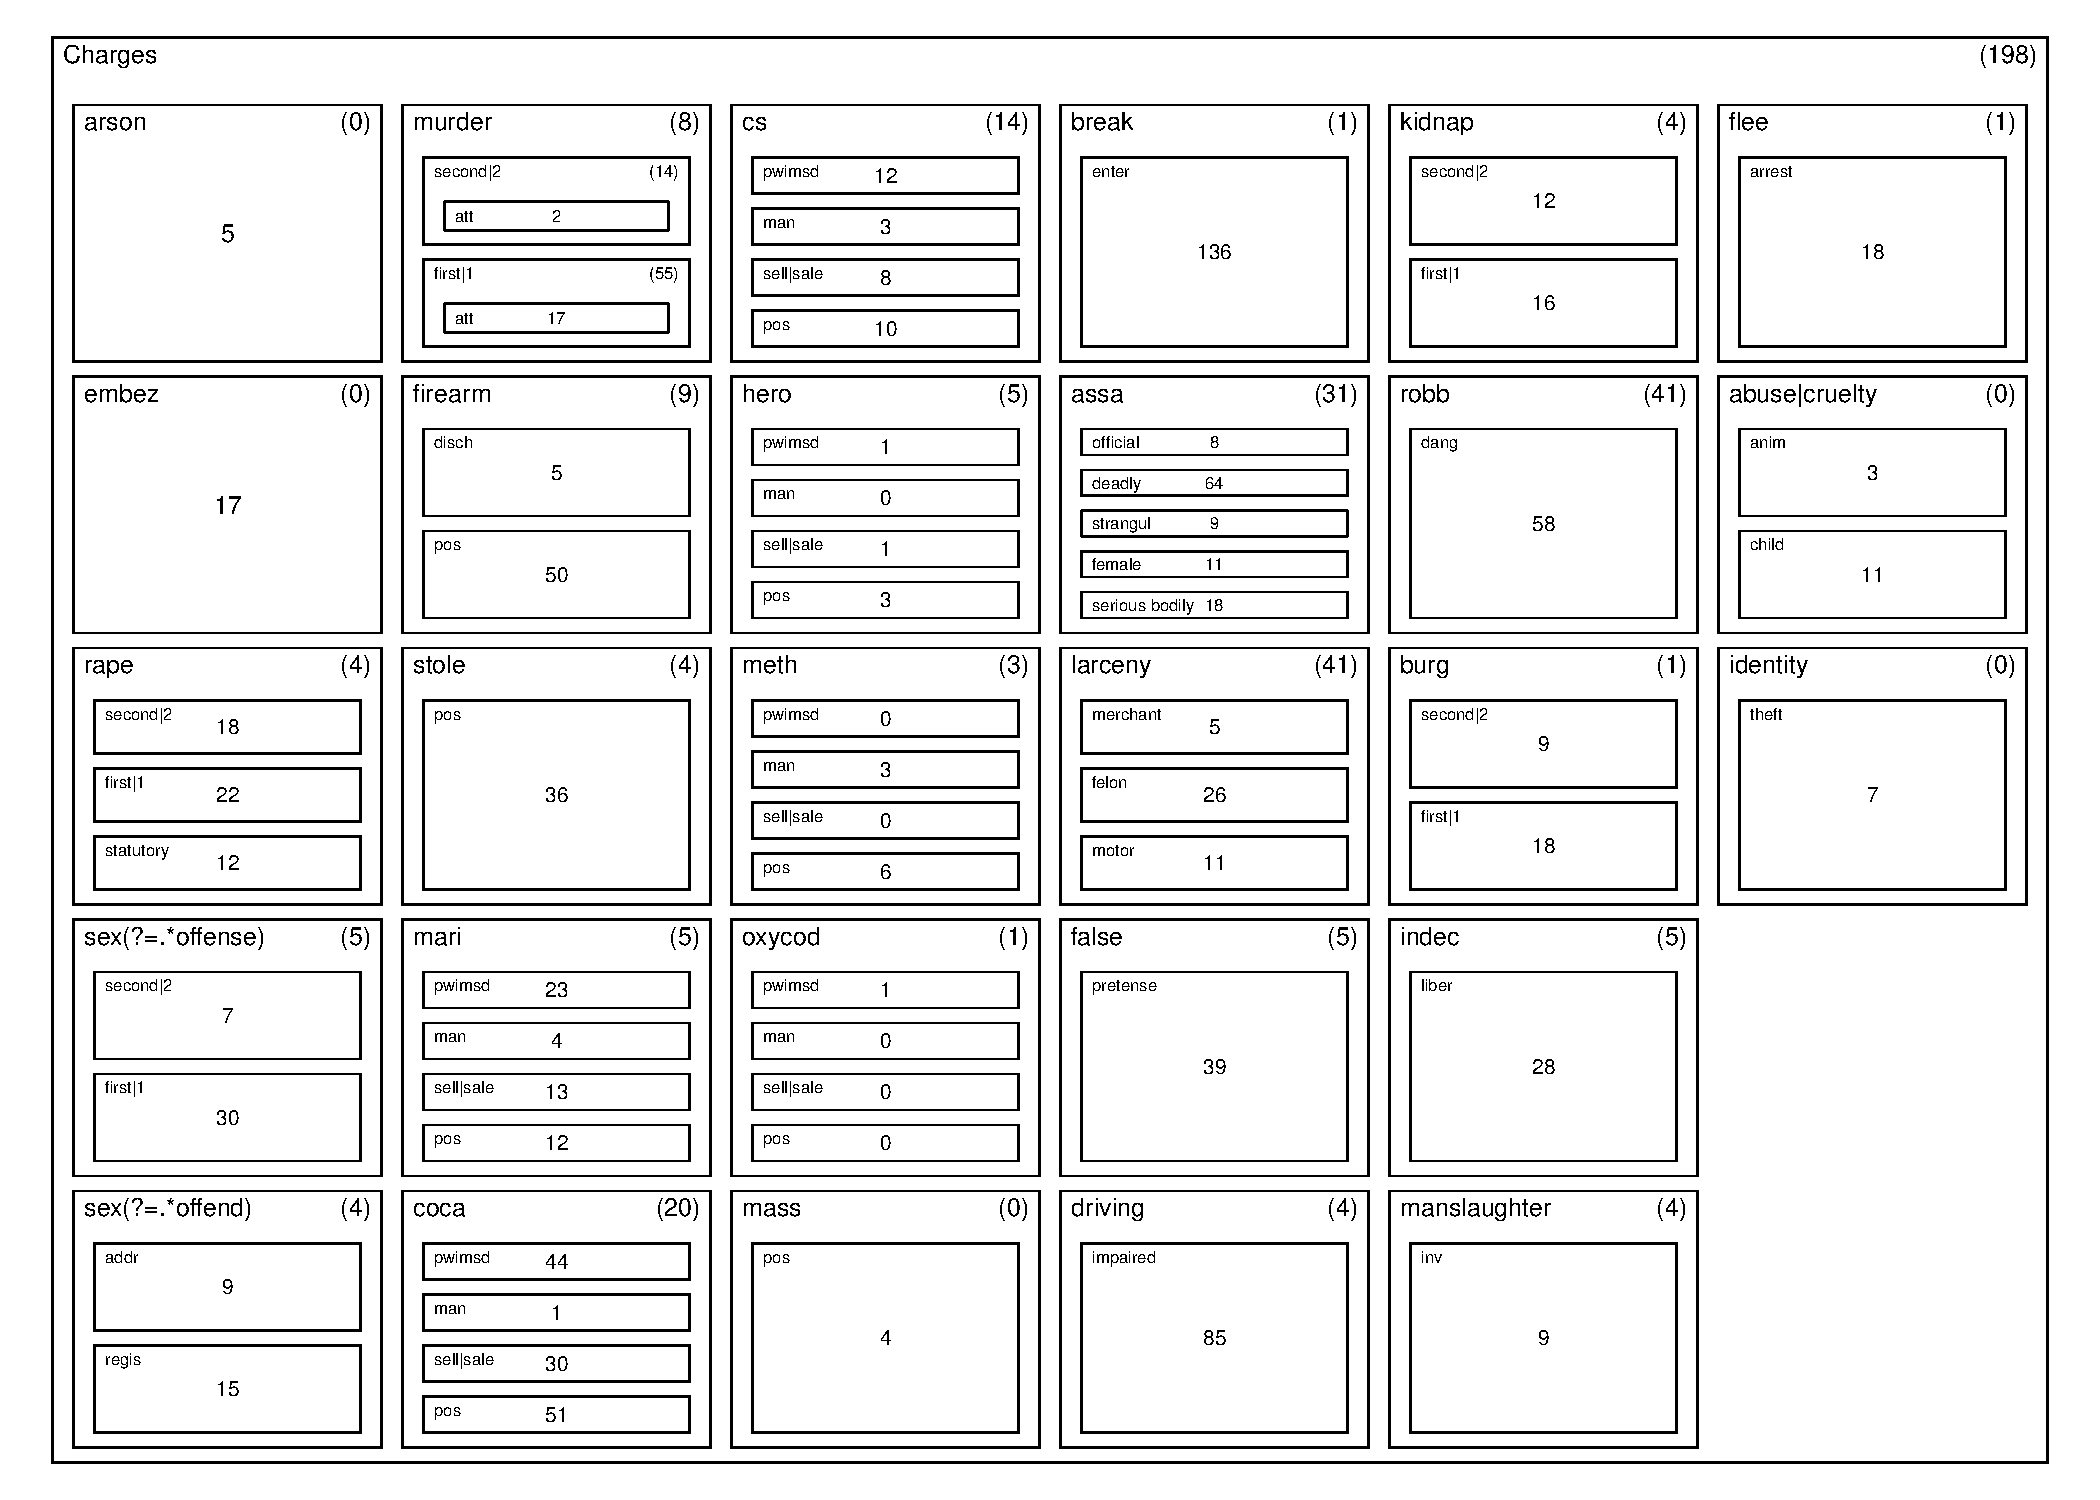
\includegraphics[angle=90, origin=c, width=1\textwidth]{ChargeDiagram}
  \caption[Regular expression charge tree visualized]{The regular expression charge tree arranged by hierarchy with counts
    provided. The counts in brackets indicate the counts of charges which could not be classified to a lower level of the
    hierarchy}
  \label{fig:chargetree}
\end{figure}

\section{Analysis Code} \label{app:analysis}

\lstinputlisting{Pictures/AnalysisScript.R}

\section{Using Sweave to include \Rp code (and more) in your report}
The easiest (and most elegant) way to include \Rp code and its output (and
have all your figures up to date with your report) is to use Sweave. You
can find an introduction Sweave in \texttt{/u/sfs/StatSoftDoc/Sweave/Sweave-tutorial.pdf}.

%%% Local Variables: 
%%% mode: latex
%%% TeX-master: "MasterThesisSfS"
%%% End: 

\chapter{Yet another appendix....}

\section{Description}
\begin{description}
\item[Something] details.
\item[Something else] other definition.
\end{description}

\section{Tables}
Refer to Table~\ref{tab:example} to see a left justified table with caption
on top.

\begin{table}[ht]
\centering
\caption[Test results]{\label{tab:example}Results.}
\begin{tabular}{ll}
\hline
\textbf{Student} & \textbf{Grade}\\
\hline
Marie  & $6$\\
Alain  & $5.5$\\
Josette  & $4.5$\\
Pierre  & $5$\\
\hline
\end{tabular}
\end{table}

%%% Local Variables: 
%%% mode: latex
%%% TeX-master: "MasterThesisSfS"
%%% End: 

\chapter{Code}
\label{app:code}

\section{Data Processing Code}\label{app:proccode}
Below is all of the code used to load and process the data, including both function definitions and the script which details the
order and method of their calling. A more convenient way of accessing the code is through the author's GitHub
(https://github.com/Salahub/peremptory\_challenges), where all of the code and some basic data files are posted.

\lstinputlisting{Pictures/DataProcess.R}

\section{Analysis Code} \label{app:analysis}
As for the data processing code, this code is more conveniently accessed using the author's GitHub
(https://github.com/Salahub/peremptory\_challenges).

\lstinputlisting{Pictures/AnalysisScript.R}



%% Epilogue (optional)
\addtocontents{toc}{\vspace{.5\baselineskip}}
\cleardoublepage
\phantomsection
\addcontentsline{toc}{chapter}{\protect\numberline{}{Epilogue}}
\markboth{Epilogue}{Epilogue}
\chapter*{Epilogue}
\label{s:Epilogue}

I came into this project broadly sceptical of the attempt to change the legal system by the removal of peremptory challenges,
fully expecting a thorough analysis to justify my distaste at the politics of the response to the verdict of
\textit{R. v. Stanley}. It is easy for a government to take action which appears good for political points before considering the
consequences. After reading the history of peremptory challenges, studying legal analyses of the practice, and viewing data for
myself, however, I am convinced that the abolition of the practice may be the best path forward. \cite{hoffman1997} was perhaps
the best argument I saw from either side of the debate, and \citeauthor{hoffman1997}'s full-throated support of the complete
abolition of peremptory challenges was incredibly influential in developing this view.

That said, as a statistician, I cannot allow myself to say that the empirical analysis in this paper proves anything. As is
generally the case with social data, there are so many possible confounders and conflicting factors that it would be easy to
mistake a pattern for something it is not. Regardless, my hope is that the visualizations presented are considered useful in the
continued investigation of this social phenomenon and others. While the solution may not be clear yet, I believe these displays
are useful visual tools to help arrive at the solution.



%%% Local Variables: 
%%% mode: latex
%%% TeX-master: "MasterThesisSfS"
%%% End: 



%%%%%%%%%%%%%%%%%%%%%%%%%%%%%%%%%%%%%%%%%%%%%%%%%% 
%%% Declaration of originality (Do not remove!)%%%
%%%%%%%%%%%%%%%%%%%%%%%%%%%%%%%%%%%%%%%%%%%%%%%%%%
%% Instructions:
%% -------------
%% fill in the empty document confirmation-originality.pdf electronically
%% print it out and sign it
%% scan it in again and save the scan in this directory with name
%% confirmation-originality-scan.pdf 
%%
%% General info on plagiarism:
%% https://www.ethz.ch/students/en/studies/performance-assessments/plagiarism.html 
\cleardoublepage
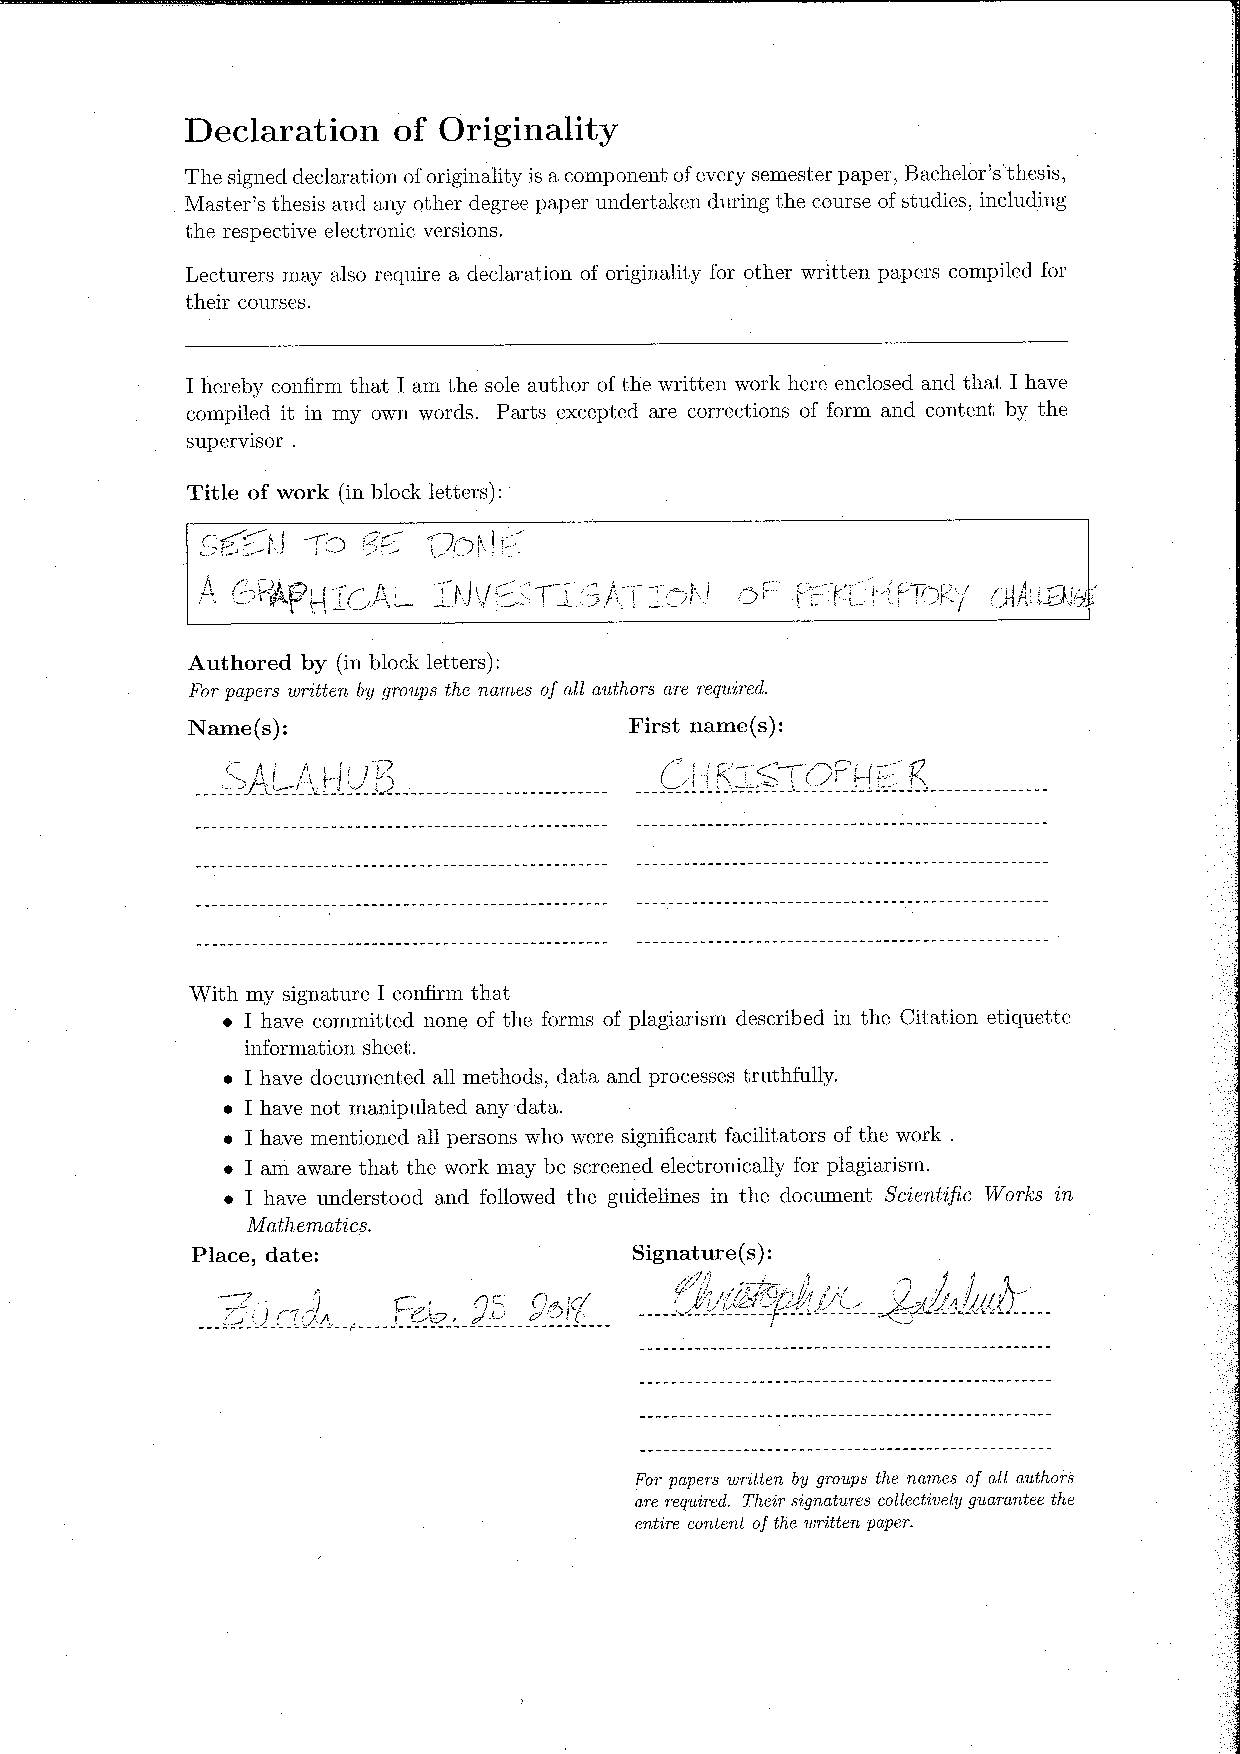
\includepdf[pages={-}, frame=true,scale=1]{confirmation-originality-scan.pdf}
\end{document}
